\subsubsection{Các dạng toán}

\subsubsubsection{Trắc nghiệm (Multiple Choice)}
Dạng bài tập trắc nghiệm cho phép người học lựa chọn một đáp án đúng trong bốn đáp án được cung cấp sẵn. Sau khi chọn đáp án, hệ thống sẽ phản hồi trực quan bằng hiệu ứng nhấp nháy hoặc đổi màu để giúp học sinh nhận biết kết quả ngay lập tức. Dạng bài này thường được sử dụng để luyện tập các phép tính cơ bản, nhận diện hình học, so sánh số hoặc các câu hỏi lý thuyết đơn giản phù hợp với học sinh tiểu học.

\begin{figure}[H]
	\centering
	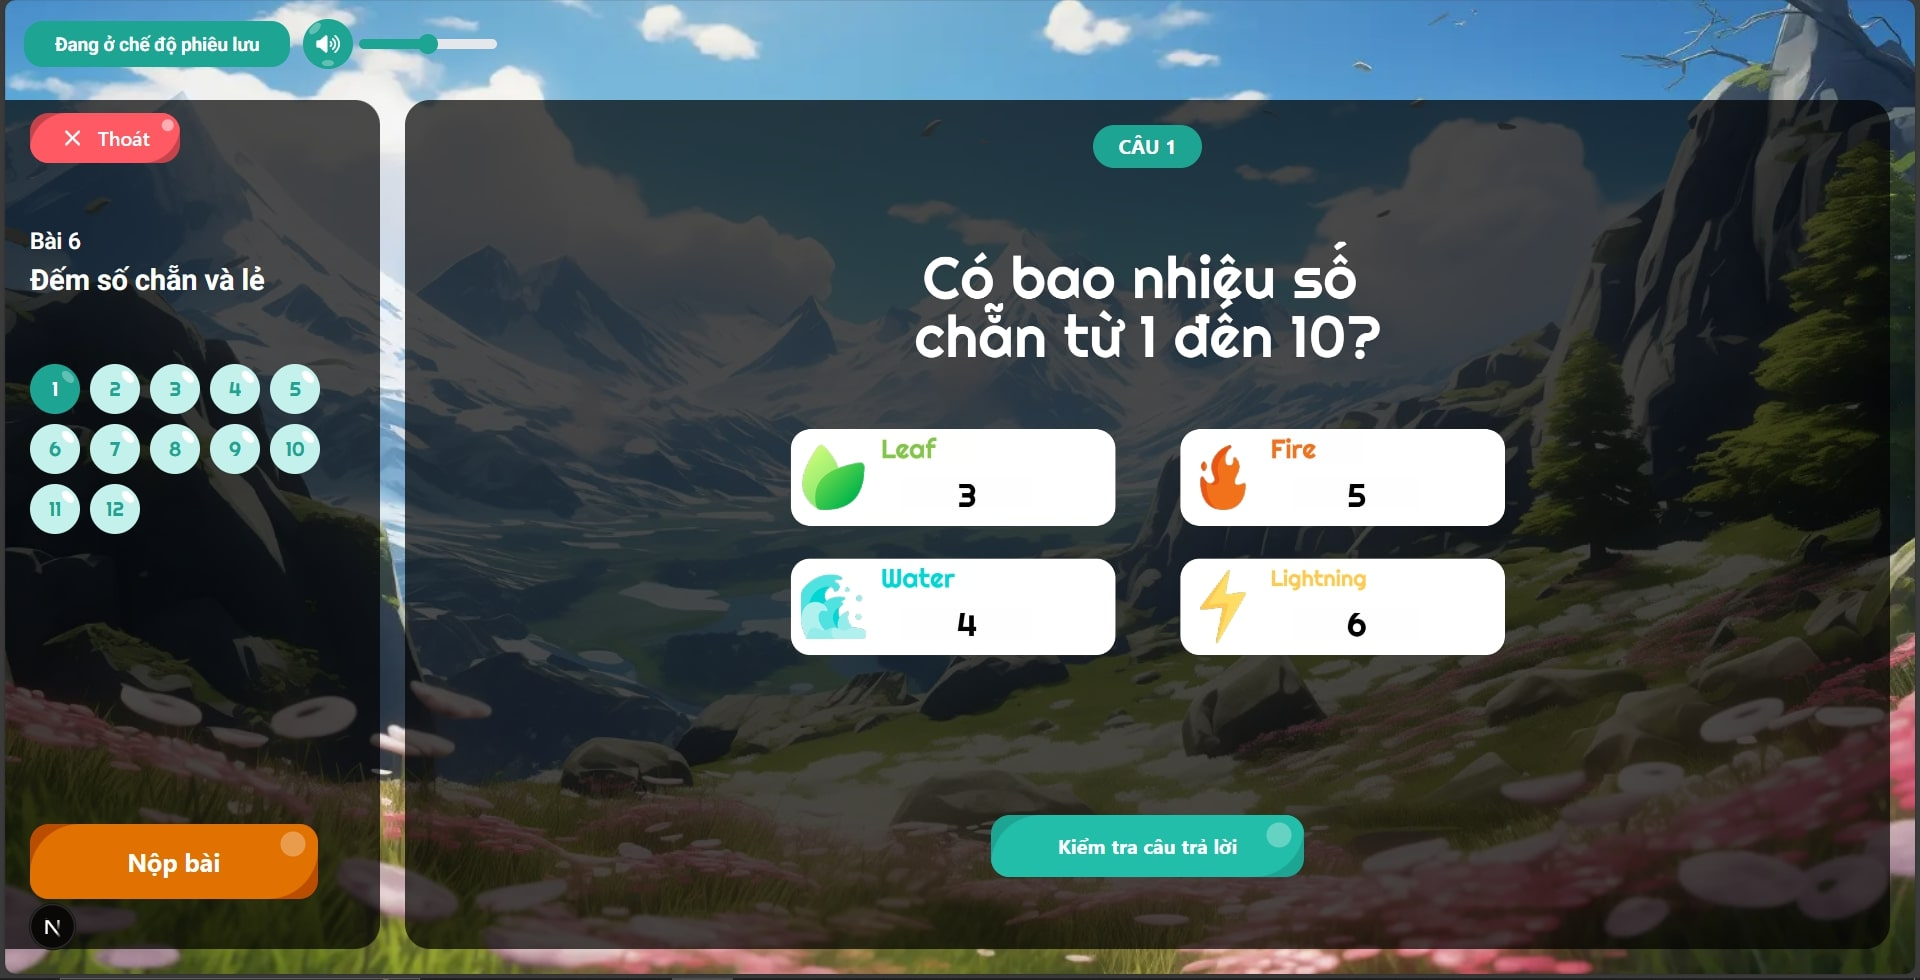
\includegraphics[width=0.9\textwidth]{Image/UI/Exercises/MultiChoice.jpg}
	\caption{Dạng bài trắc nghiệm}
	\label{fig:multiple-choice}
\end{figure}

\subsubsubsection{Ghép cặp (Matching)}
Trong dạng bài ghép cặp, người học thực hiện thao tác kéo thả để nối các đối tượng tương ứng với nhau, ví dụ như phép tính với kết quả tương ứng. Khi ghép đúng, các đối tượng sẽ đổi màu hoặc xuất hiện hiệu ứng phản hồi nhằm tăng tính trực quan và tạo cảm giác hứng thú trong quá trình học tập.

\begin{figure}[H]
	\centeringMô 
	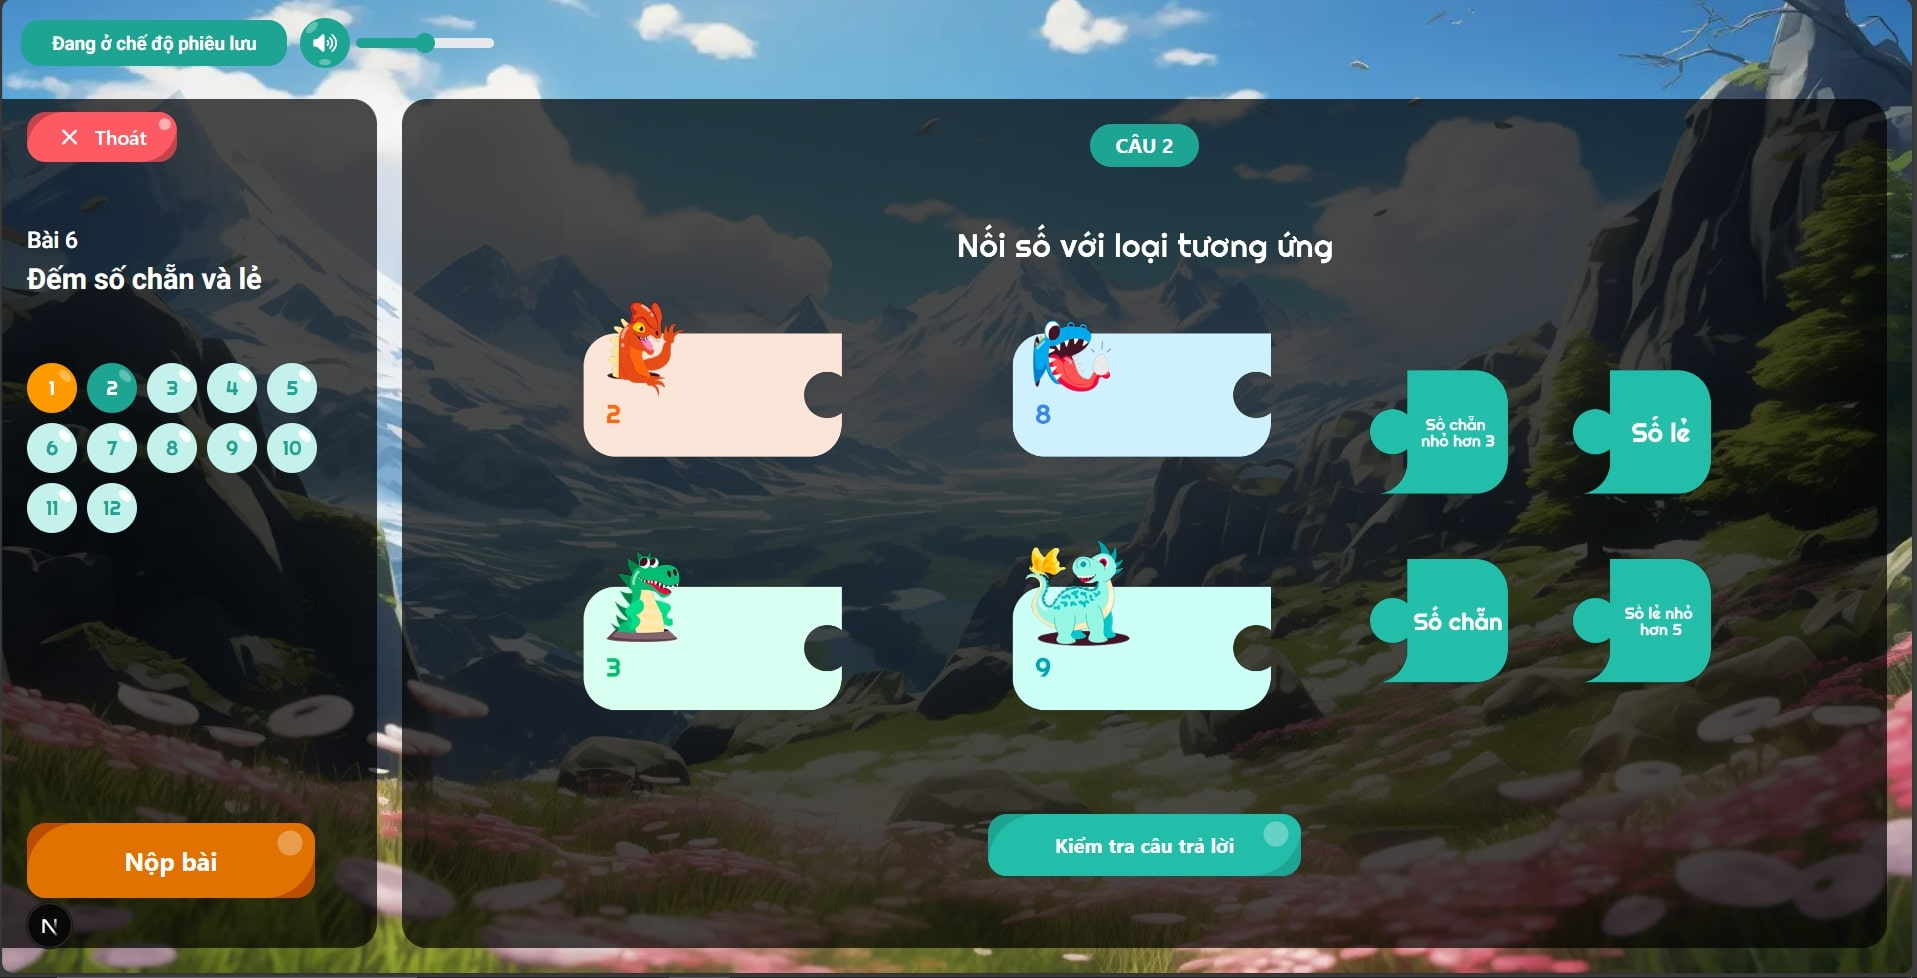
\includegraphics[width=0.9\textwidth]{Image/UI/Exercises/Matching.jpg}
	\caption{Dạng bài ghép cặp}
	\label{fig:matching}
\end{figure}

\subsubsubsection{Điền số (Fill in the Blanks)}
Dạng bài điền số yêu cầu học sinh nhập giá trị thích hợp vào các ô trống trong biểu thức hoặc câu hỏi toán học. Một bài có thể chứa tối đa ba ô trống và hệ thống sẽ chấm điểm độc lập cho từng phần nhằm hỗ trợ đánh giá chính xác hơn. Dạng bài này giúp rèn luyện khả năng tính toán và tư duy từng bước của người học.

\begin{figure}[H]
	\centering
	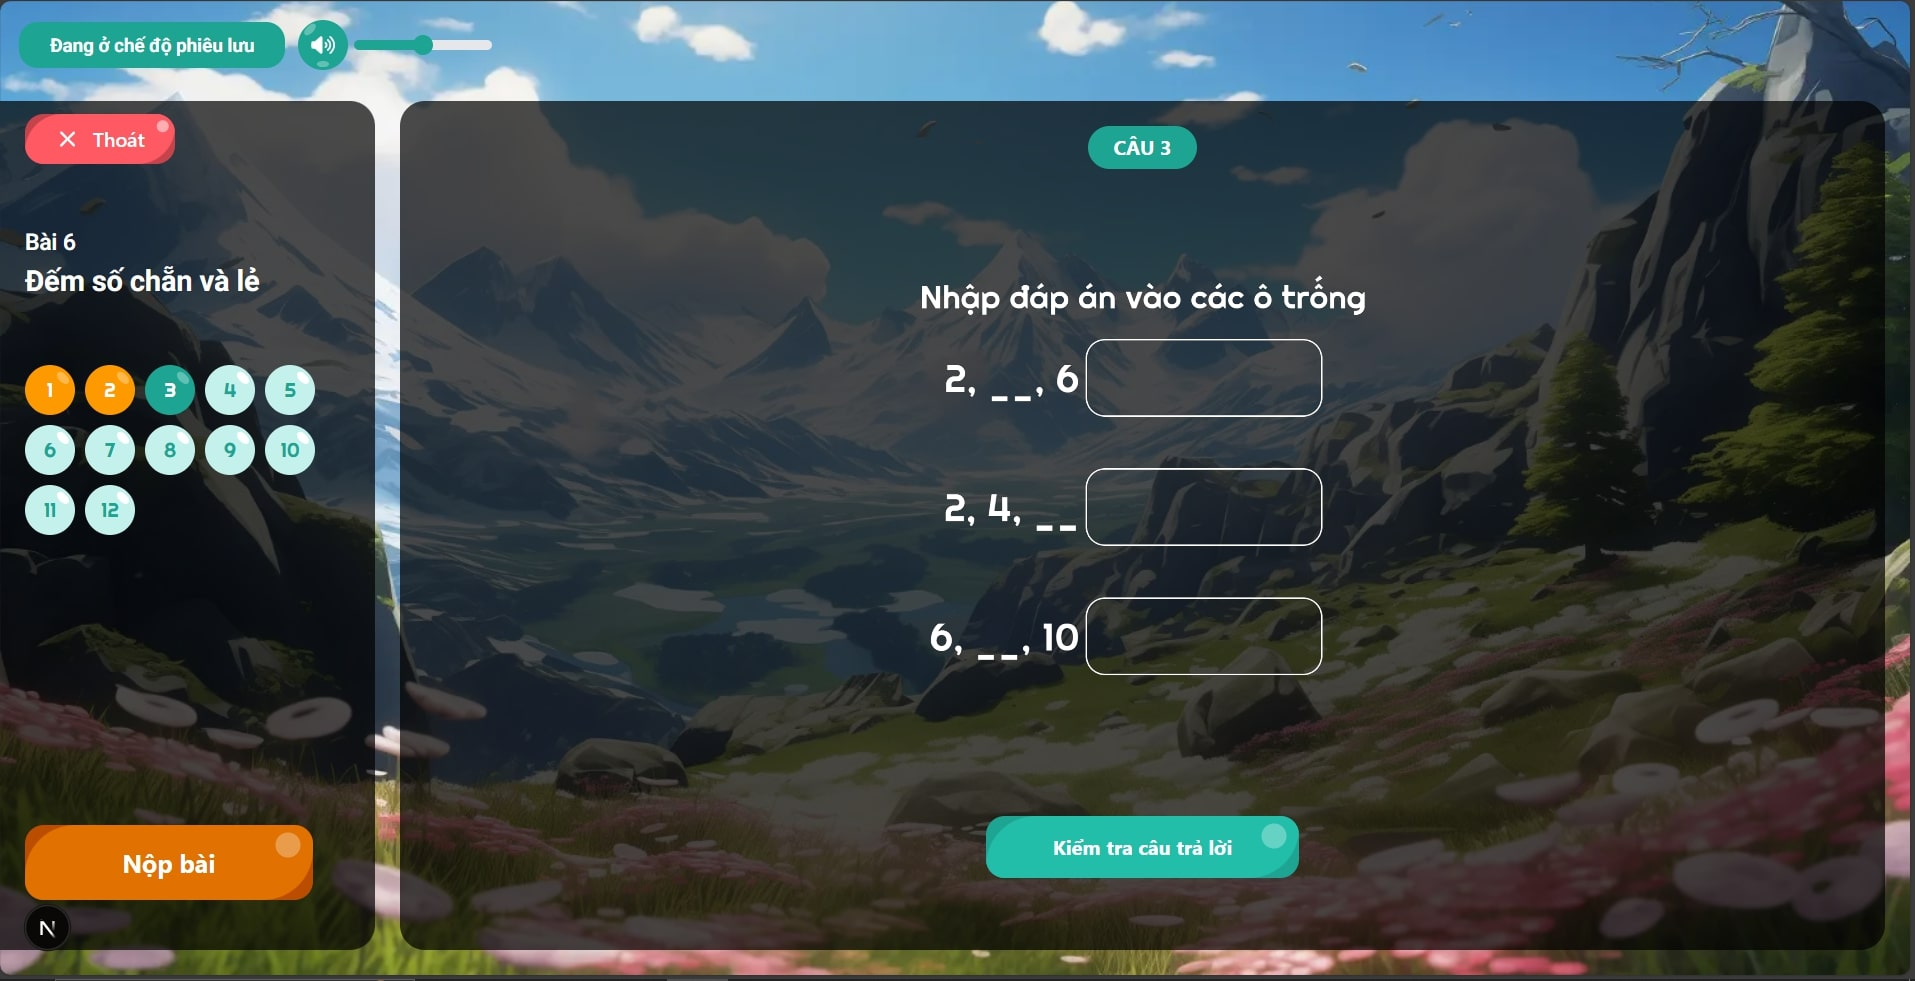
\includegraphics[width=0.9\textwidth]{Image/UI/Exercises/Fill.jpg}
	\caption{Dạng bài điền số}
	\label{fig:fill}
\end{figure}

\subsubsubsection{Kéo thả (Drag and Drop)}
Ở dạng bài này, người học sẽ kéo các con số hoặc ký hiệu toán học vào đúng vị trí còn thiếu trong biểu thức. Nếu thả sai vị trí, hệ thống sẽ tự động đưa đối tượng trở về vị trí ban đầu để người học thử lại. Cơ chế tương tác trực tiếp giúp học sinh dễ dàng tiếp cận và ghi nhớ các phép tính cơ bản.

\begin{figure}[H]
	\centering
	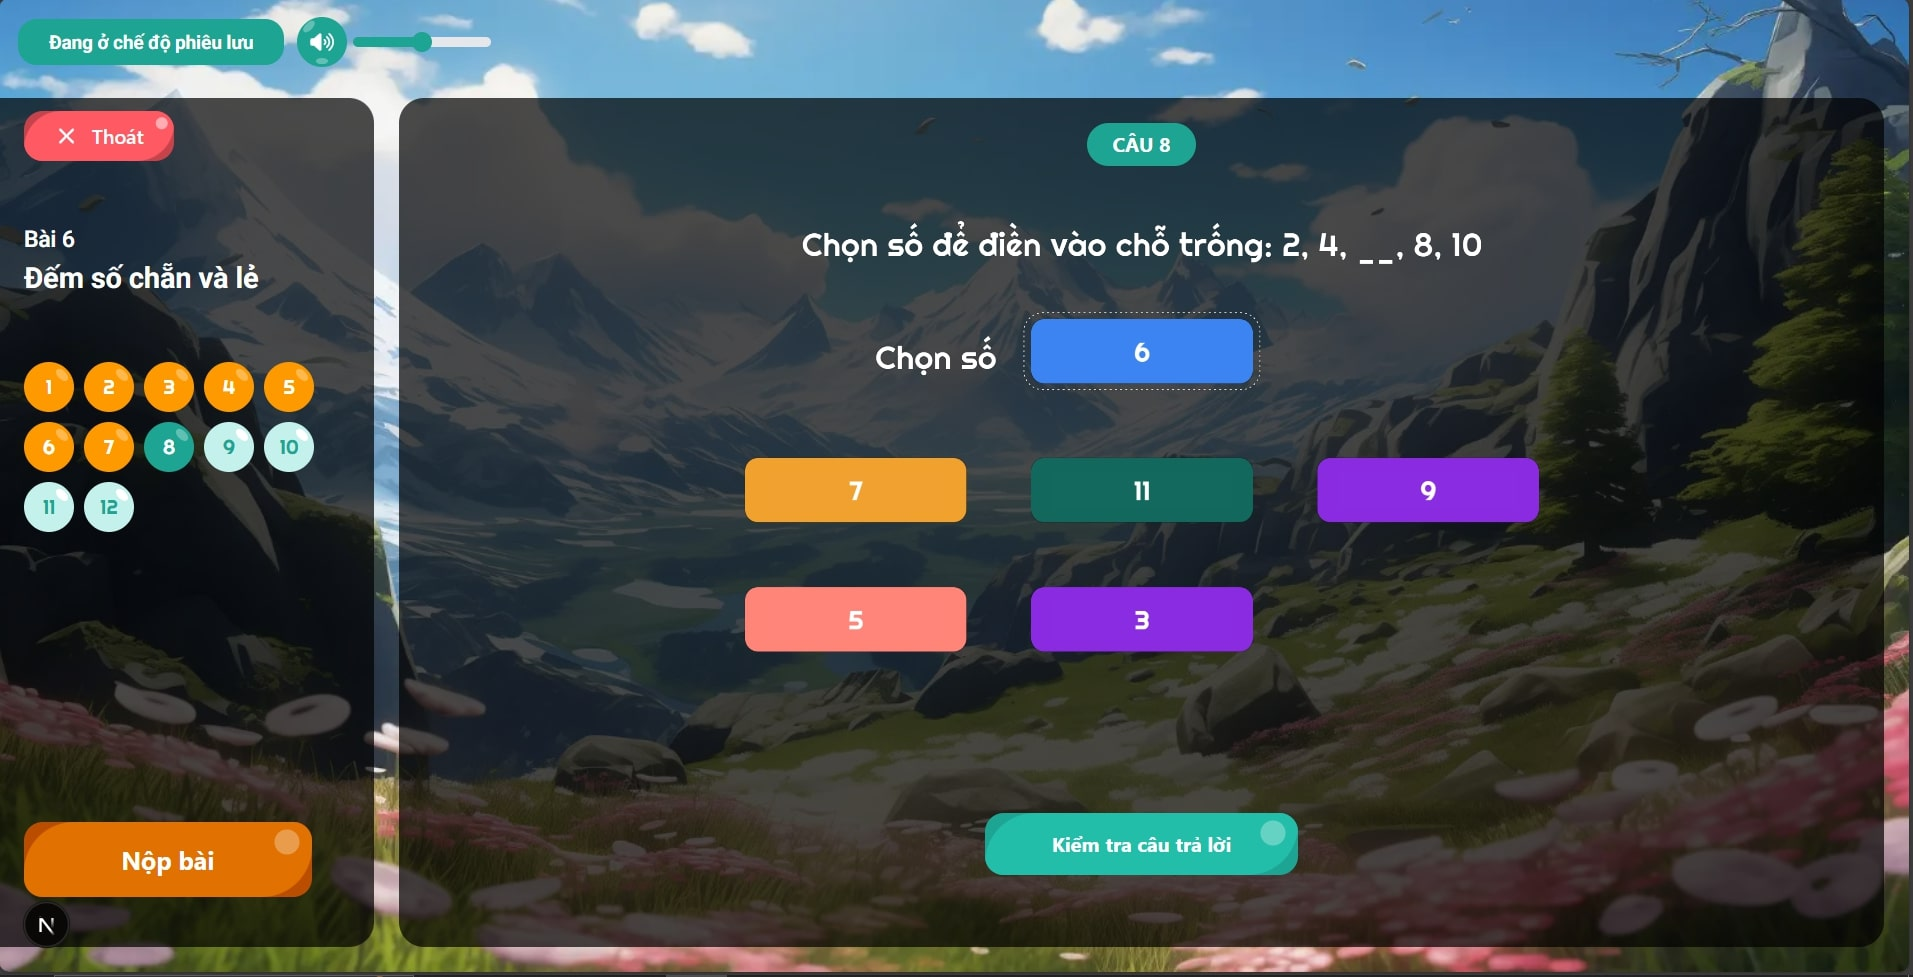
\includegraphics[width=0.9\textwidth]{Image/UI/Exercises/Drag.jpg}
	\caption{Dạng bài kéo thả}
	\label{fig:drag}
\end{figure}

\subsubsubsection{Phân loại chẵn/lẻ (Grouping)}
Dạng bài phân loại yêu cầu học sinh lựa chọn chế độ phân loại trước khi bắt đầu làm bài, trong đó số chẵn được biểu diễn bằng màu xanh và số lẻ được biểu diễn bằng màu hồng. Sau khi chọn chế độ, người học sẽ click trực tiếp vào từng con số để tô màu tương ứng, tương tự như một trò chơi tô màu tương tác. Hệ thống chỉ kiểm tra kết quả sau khi hoàn thành toàn bộ thao tác, giúp học sinh tập trung vào quá trình quan sát, suy luận và tự đánh giá trước khi nộp đáp án.

\begin{figure}[H]
	\centering
	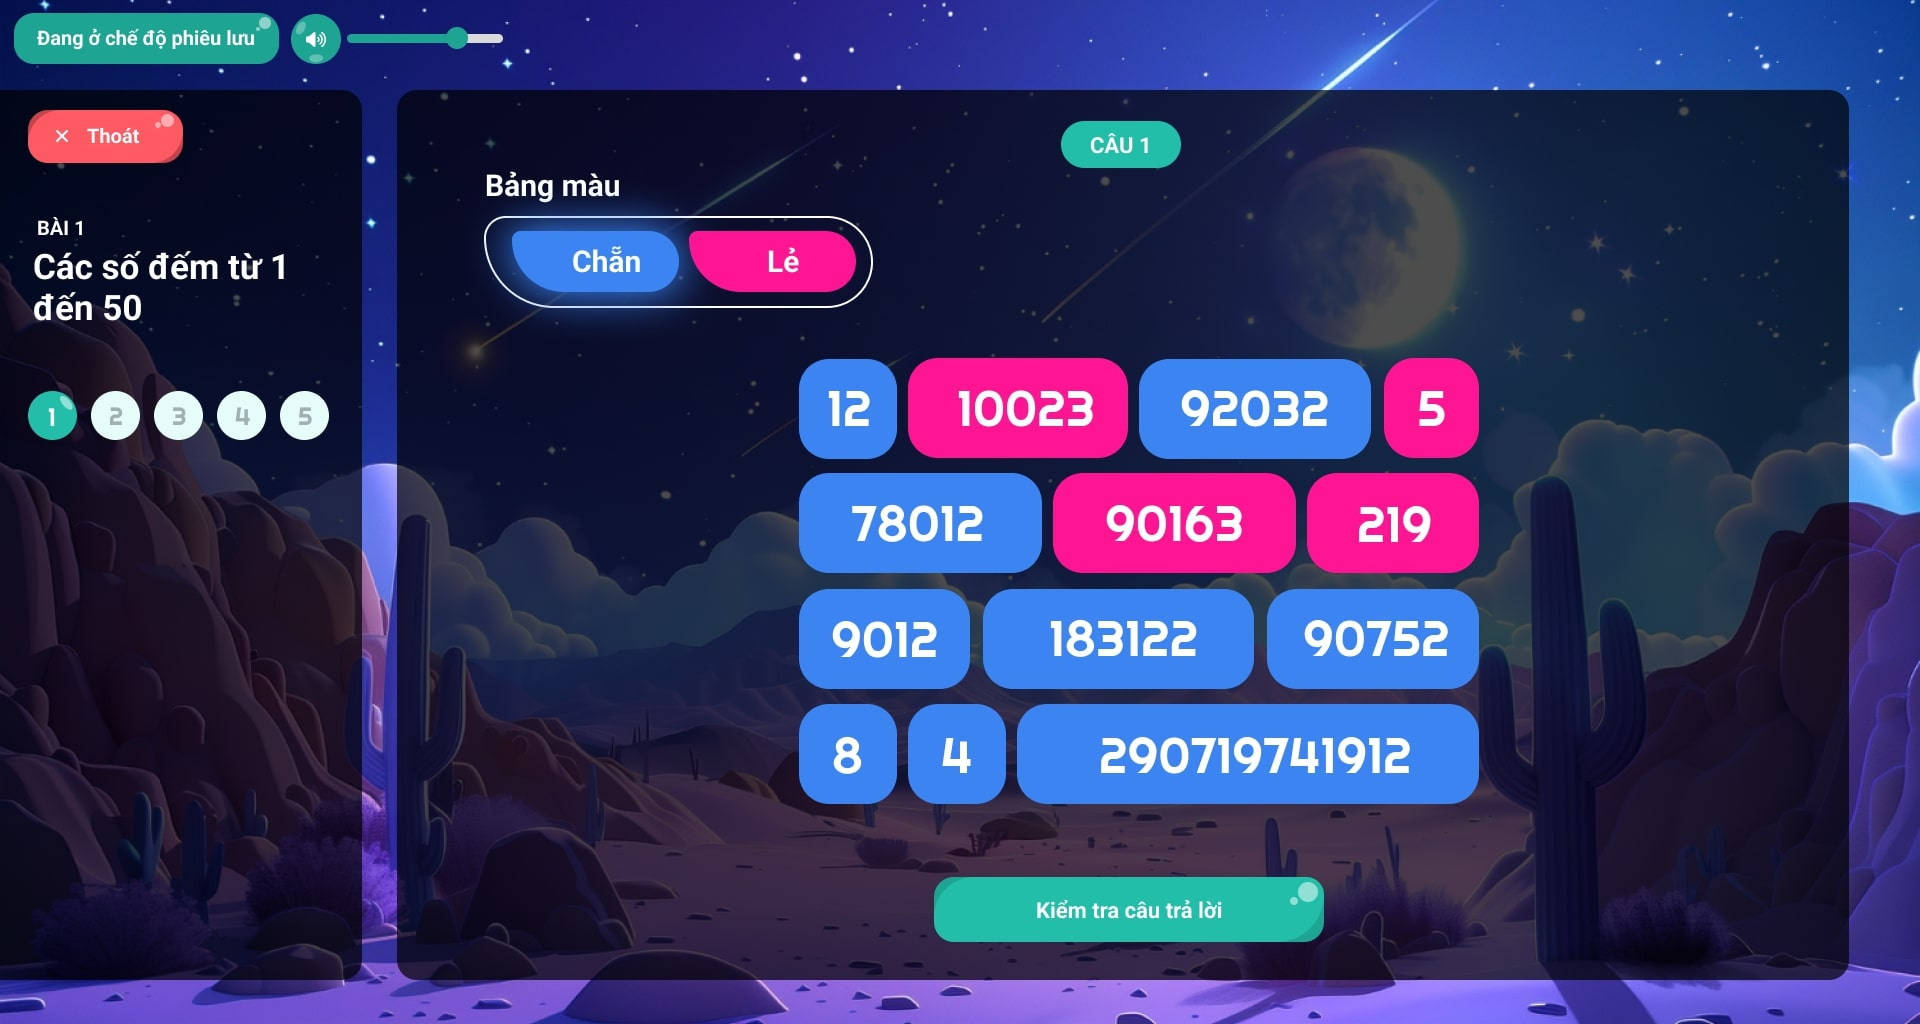
\includegraphics[width=0.9\textwidth]{Image/UI/Exercises/Grouping.jpg}
	\caption{Dạng bài phân loại}
	\label{fig:grouping}
\end{figure}

\subsubsubsection{Đúng/Sai (True/False)}
Dạng bài đúng/sai cung cấp cho người học một mệnh đề hoặc phép tính và yêu cầu lựa chọn “Đúng” hoặc “Sai”. Hệ thống chỉ cho phép một lựa chọn duy nhất nhằm đảm bảo tính rõ ràng trong câu trả lời. Đây là dạng bài đơn giản nhưng hiệu quả trong việc kiểm tra khả năng nhận biết nhanh và tư duy logic của học sinh.

\begin{figure}[H]
	\centering
	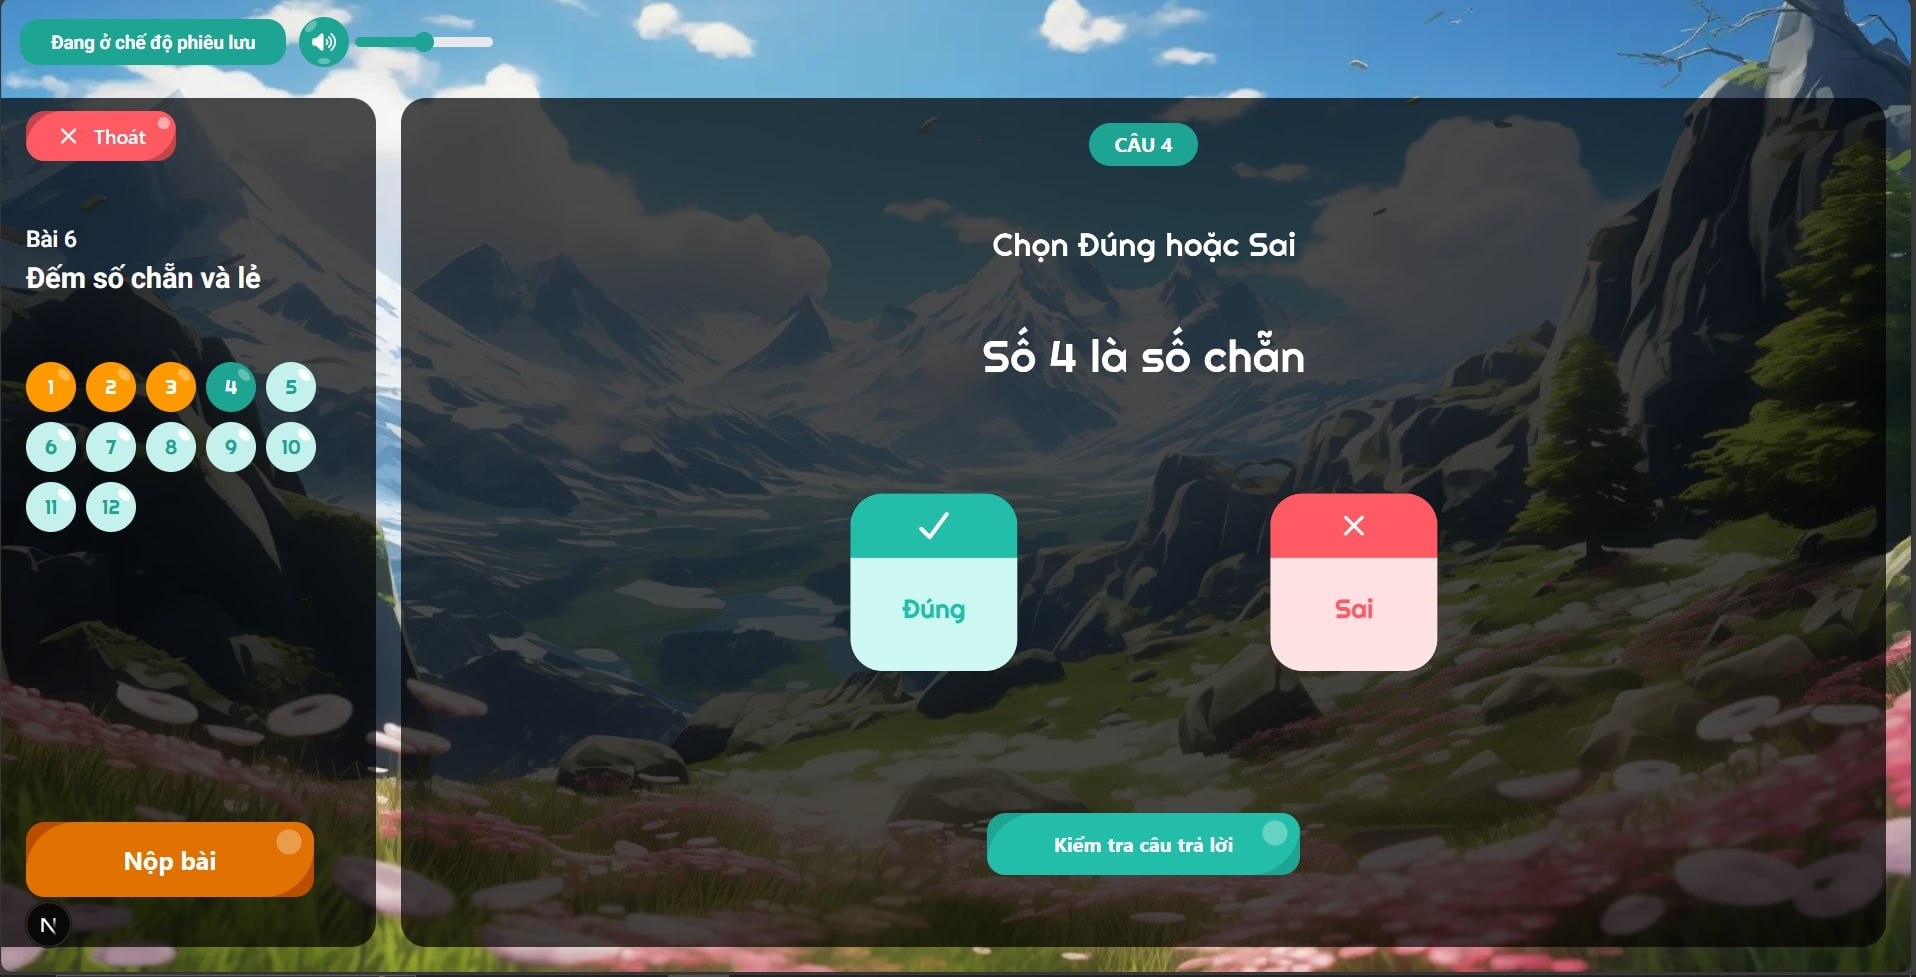
\includegraphics[width=0.9\textwidth]{Image/UI/Exercises/TrueFalse.jpg}
	\caption{Dạng bài đúng/sai}
	\label{fig:truefalse}
\end{figure}

\subsubsubsection{Tổ hợp burger (Burger)}
Dạng bài tổ hợp burger giúp học sinh làm quen với tư duy tổ hợp và lựa chọn thành phần theo yêu cầu đề bài. Hệ thống cung cấp bốn loại nguyên liệu gồm cà chua, thịt, phô mai và rau. Dựa trên yêu cầu của bài toán, người học cần lựa chọn và sắp xếp đúng các nguyên liệu để tạo ra chiếc burger phù hợp. Một bài toán có thể có nhiều cách tạo burger khác nhau miễn đáp ứng đúng yêu cầu về thành phần.

\begin{figure}[H]
	\centering
	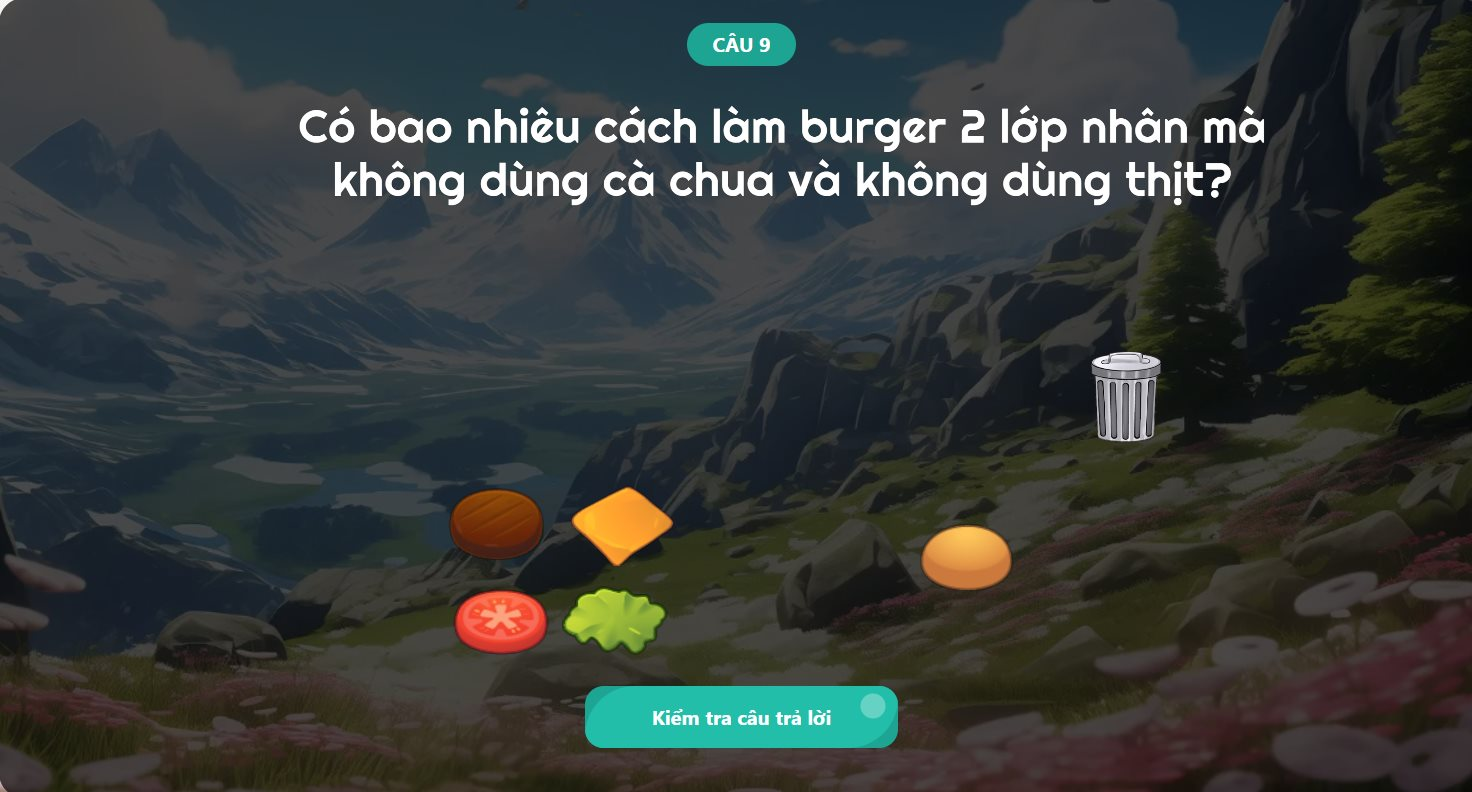
\includegraphics[width=0.9\textwidth]{Image/UI/Exercises/Burger.jpg}
	\caption{Dạng bài tổ hợp burger}
	\label{fig:burger}
\end{figure}

\subsubsubsection{Xe buýt (Bus)}
Dạng bài xe buýt được xây dựng nhằm giúp học sinh hiểu rõ giá trị hàng đơn vị, hàng chục và hàng trăm. Hệ thống cung cấp ba loại hộp tương ứng với giá trị 1, 10 và 100. Theo yêu cầu bài toán, học sinh cần lựa chọn các hộp sao cho tổng giá trị đúng với số lượng cần vận chuyển. Ví dụ, để vận chuyển 100 linh kiện, học sinh có thể chọn một hộp 100 hoặc mười hộp 10. Khi chọn hộp, các hộp sẽ bay trực tiếp lên xe buýt tạo nên trải nghiệm học tập sinh động và trực quan.

\begin{figure}[H]
	\centering
	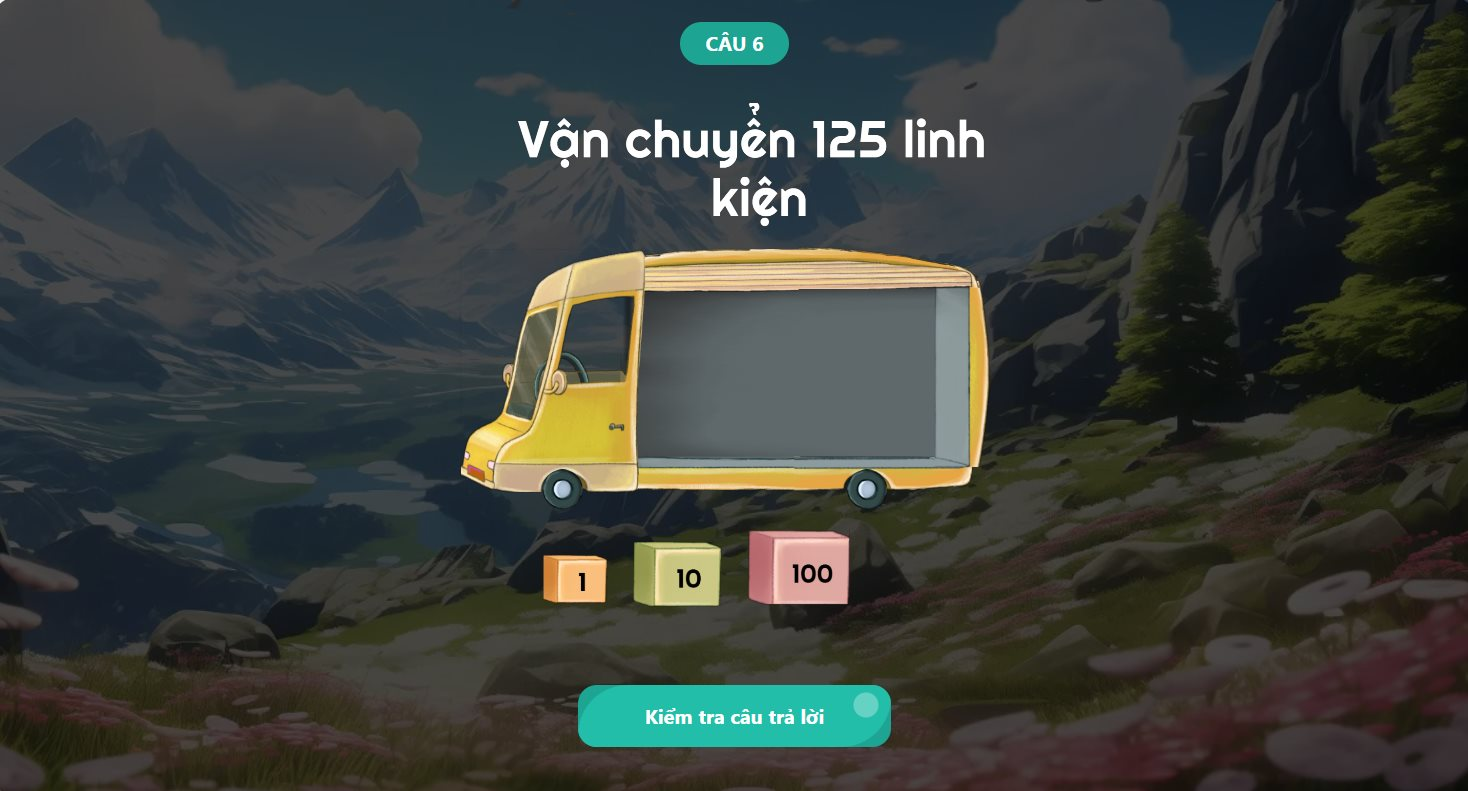
\includegraphics[width=0.9\textwidth]{Image/UI/Exercises/Bus.jpg}
	\caption{Dạng bài xe buýt}
	\label{fig:bus}
\end{figure}

\subsubsubsection{Bắt chim (Catch Bird)}
Trong dạng bài bắt chim, trên cây sẽ có một số lượng chim ban đầu và người học cần click vào các chú chim để chúng bay vào lồng. Số lượng chim trong lồng sẽ đại diện cho kết quả của bài toán. Nhờ cơ chế biểu diễn trực quan này, hệ thống có thể mở rộng thành nhiều dạng câu hỏi khác nhau.

\begin{figure}[H]
	\centering
	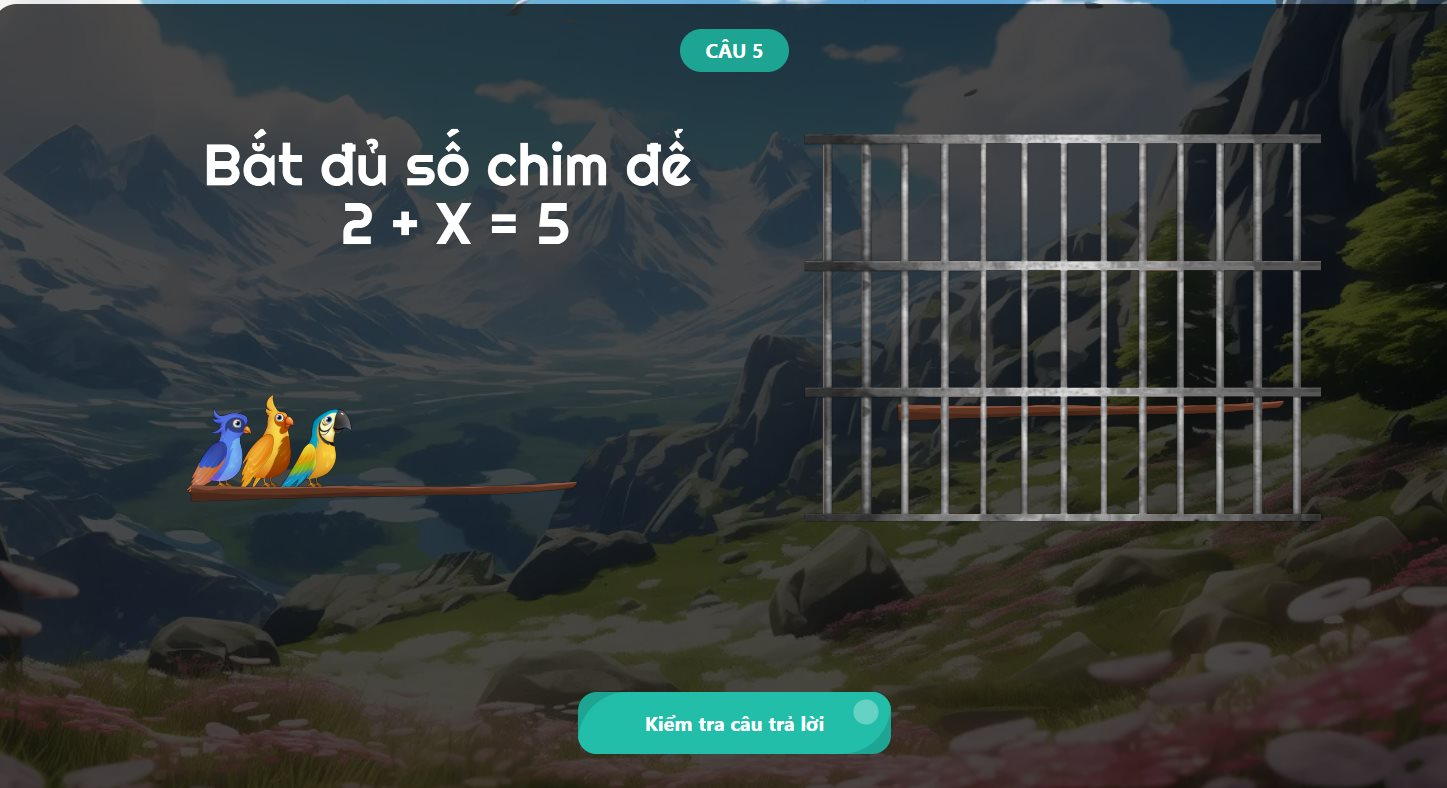
\includegraphics[width=0.9\textwidth]{Image/UI/Exercises/CatchBird.jpg}
	\caption{Dạng bài bắt chim}
	\label{fig:catchbird}
\end{figure}

\subsubsubsection{Đồng hồ (Clock)}
Dạng bài đồng hồ giúp học sinh học cách xem giờ thông qua đồng hồ kim 12 giờ. Người học cần xoay kim đồng hồ đến đúng thời gian được yêu cầu. Điểm đặc biệt của dạng bài này là hệ thống có thêm khung cửa sổ mô phỏng thời gian ngày và đêm. Ví dụ, khi chỉnh đến 12 giờ trưa, khung cửa sổ sẽ hiển thị mặt trời và bầu trời sáng; ngược lại khi chỉnh đến 12 giờ đêm, cửa sổ sẽ hiển thị bầu trời tối cùng mặt trăng. Điều này giúp học sinh phân biệt rõ khái niệm hệ thống giờ 12 giờ và 24 giờ một cách trực quan và sinh động hơn

\begin{figure}[H]
	\centering
	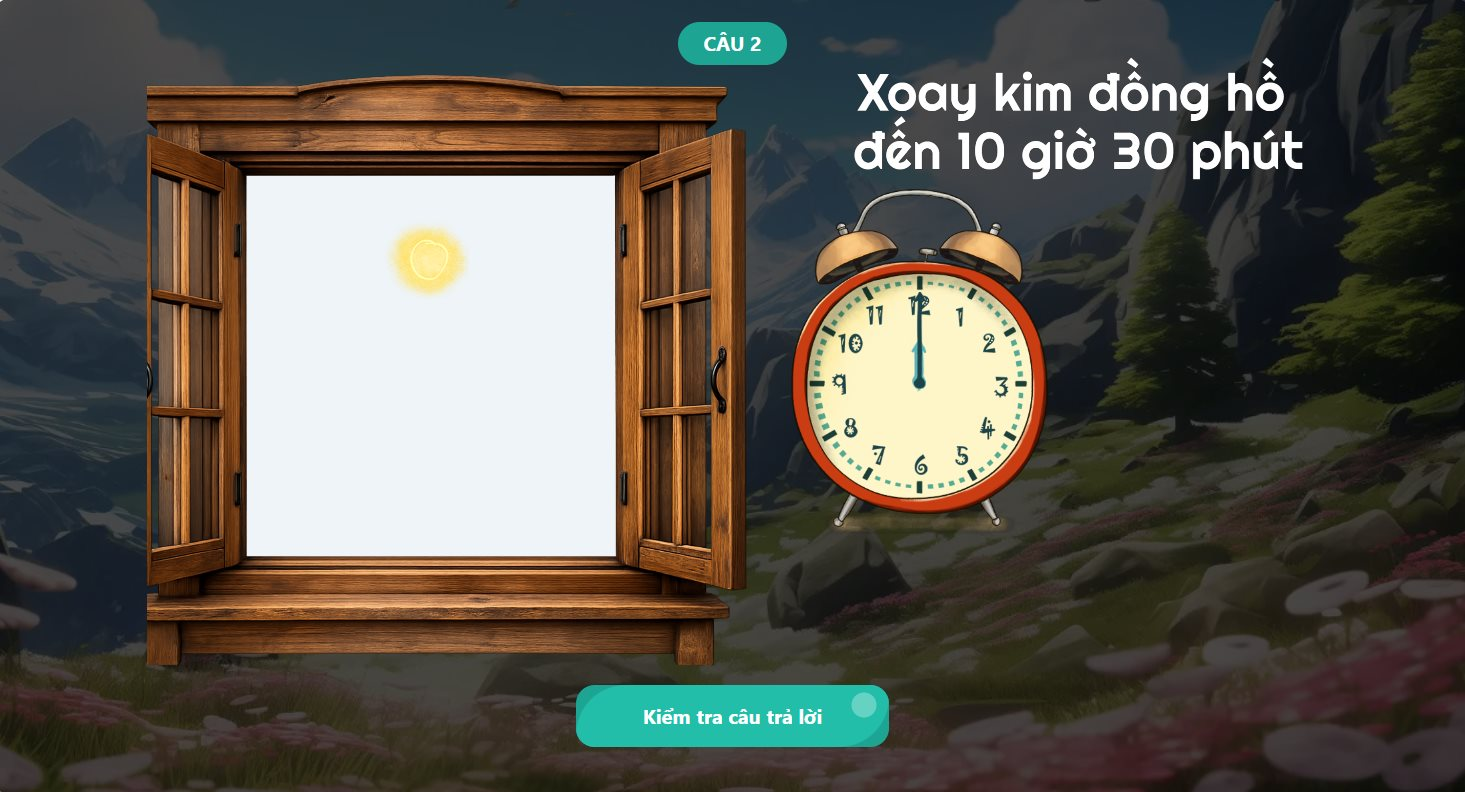
\includegraphics[width=0.9\textwidth]{Image/UI/Exercises/Clock.jpg}
	\caption{Dạng bài đồng hồ}
	\label{fig:clock}
\end{figure}

\subsubsubsection{Đổi tiền xu (Coin)}
Dạng bài đổi tiền xu hỗ trợ học sinh làm quen với giá trị tiền tệ thông qua cơ chế đổi tiền trực quan. Hệ thống cung cấp ba loại đồng xu có giá trị 1 đồng, 10 đồng và 100 đồng cùng với một máy đổi tiền. Khi đưa một đồng xu vào máy, hệ thống sẽ tự động đổi sang các đồng xu có giá trị nhỏ hơn, ví dụ một đồng 100 sẽ đổi thành mười đồng 10. Người học cần vận dụng cơ chế đổi tiền để tạo đúng số tiền theo yêu cầu của bài toán.

\begin{figure}[H]
	\centering
	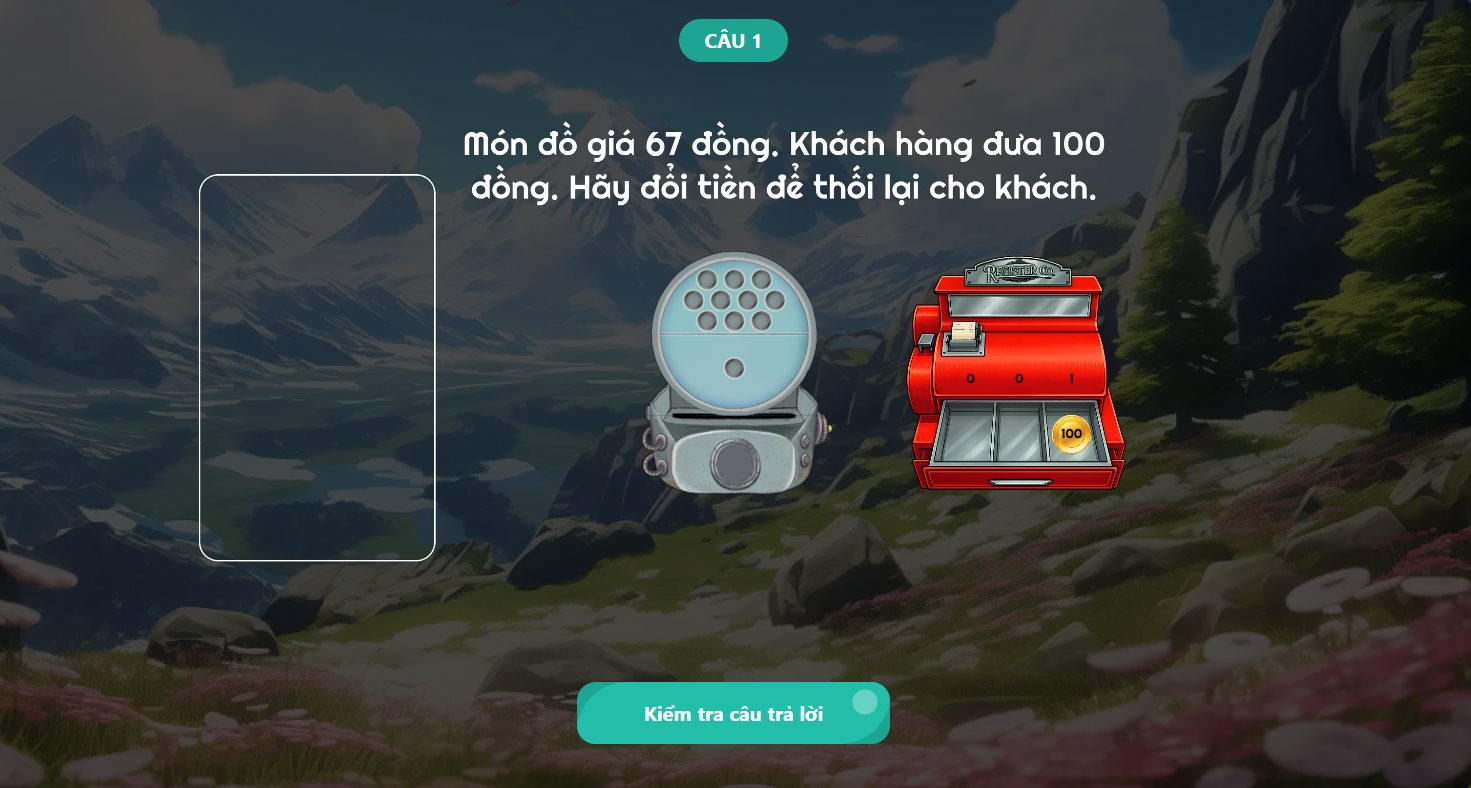
\includegraphics[width=0.9\textwidth]{Image/UI/Exercises/Coin.jpg}
	\caption{Dạng bài đổi tiền xu}
	\label{fig:coin}
\end{figure}

\subsubsubsection{Viên bi (Gumball)}
Dạng bài viên bi được thiết kế nhằm hỗ trợ học sinh luyện tập kỹ năng đếm và so sánh số lượng. Ban đầu hệ thống cung cấp một số lượng bi xanh và bi cam nhất định. Khi người học chọn một chiếc lọ, chiếc lọ sẽ di chuyển vào máy để hứng bi rơi xuống. Mỗi lần máy sẽ thả 10 viên bi và mỗi lọ chứa đúng 10 viên. Học sinh cần quan sát số lọ đã đầy cùng số viên còn lại để trả lời các câu hỏi so sánh như màu nào nhiều hơn hoặc ít hơn.

\begin{figure}[H]
	\centering
	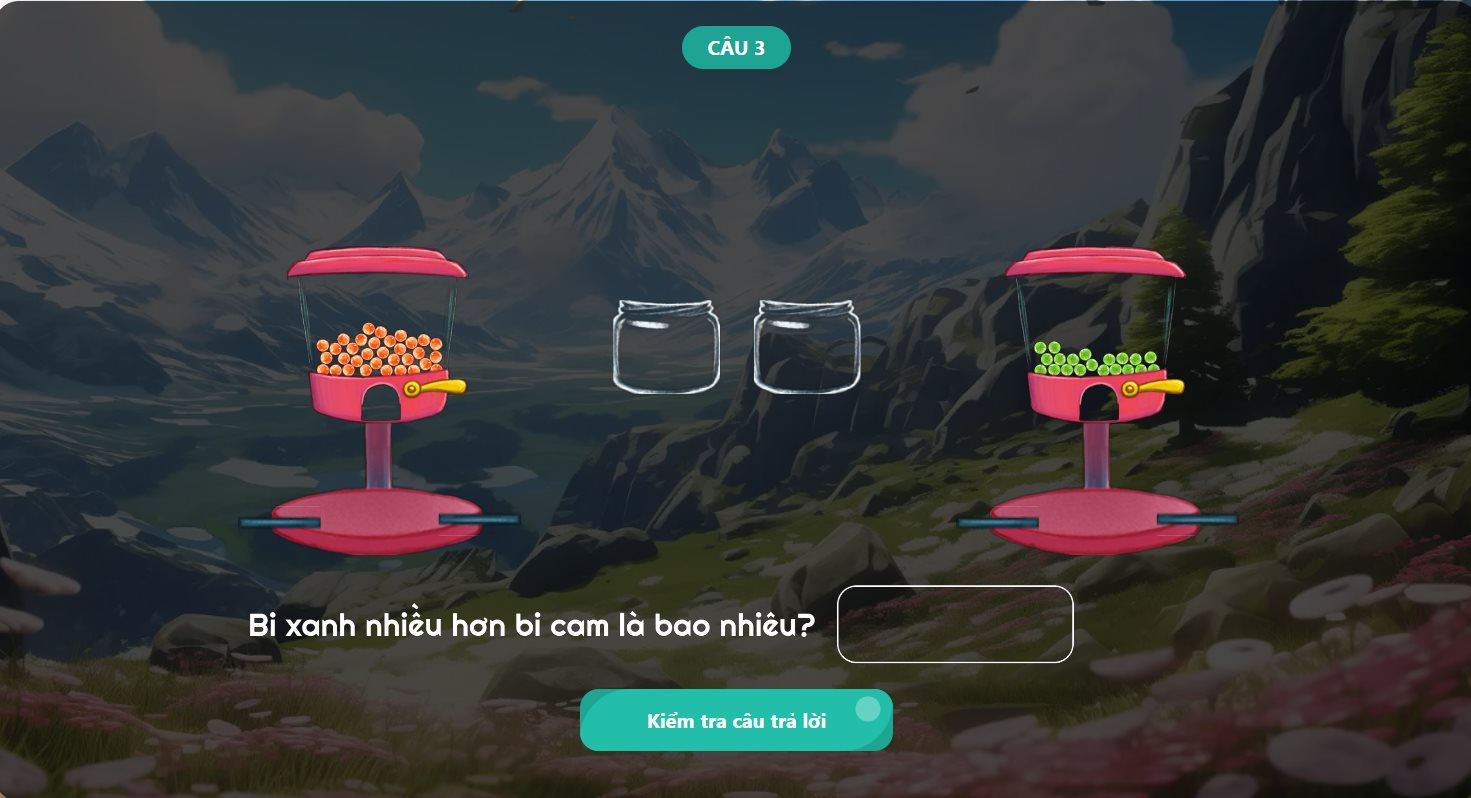
\includegraphics[width=0.9\textwidth]{Image/UI/Exercises/Gumball.jpg}
	\caption{Dạng bài viên bi}
	\label{fig:gumball}
\end{figure}

\subsubsubsection{Cân thủ công (Manual Scale)}
Dạng bài cân thủ công sử dụng mô hình cân đòn nhằm giúp học sinh làm quen với các khái niệm lớn hơn, bé hơn và bằng nhau. Người học sẽ kéo các bát hạt lên hai bên cân theo yêu cầu của đề bài. Dựa vào độ nghiêng của cân sang trái hoặc phải, học sinh có thể trực quan nhận biết mối quan hệ giữa hai giá trị.

\begin{figure}[H]
	\centering
	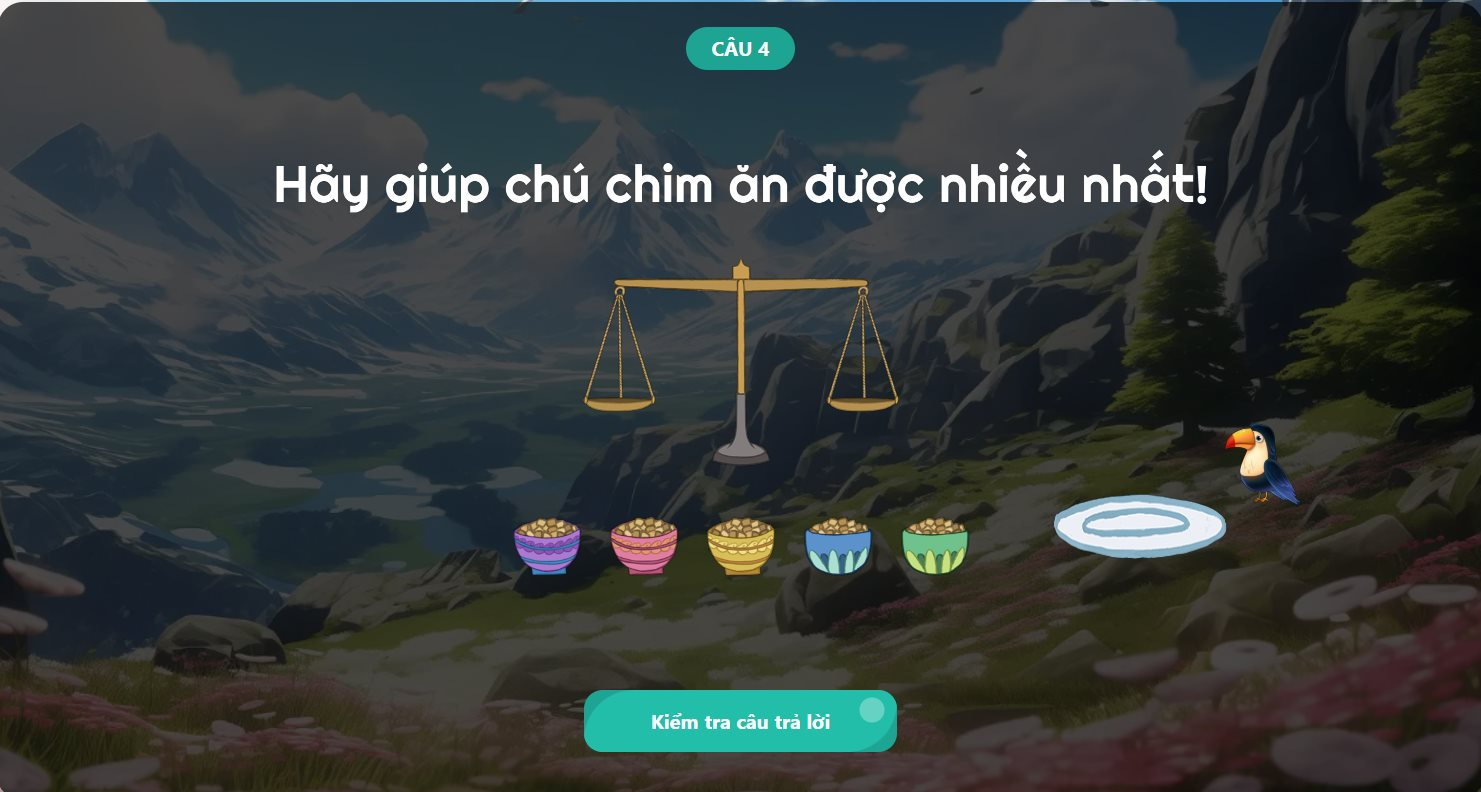
\includegraphics[width=0.9\textwidth]{Image/UI/Exercises/ManualScale.jpg}
	\caption{Dạng bài cân thủ công}
	\label{fig:manual-scale}
\end{figure}

\subsubsubsection{Chia pizza (Pizza)}
Dạng bài chia pizza giúp học sinh bước đầu làm quen với phân số thông qua việc chia chiếc pizza thành nhiều phần bằng nhau. Mỗi lát pizza sẽ có một loại topping khác nhau và bài toán sẽ yêu cầu người học tạo đúng số lượng lát tương ứng với từng loại. Dạng bài này giúp học sinh hình dung trực quan khái niệm phân số trong toán học.

\begin{figure}[H]
	\centering
	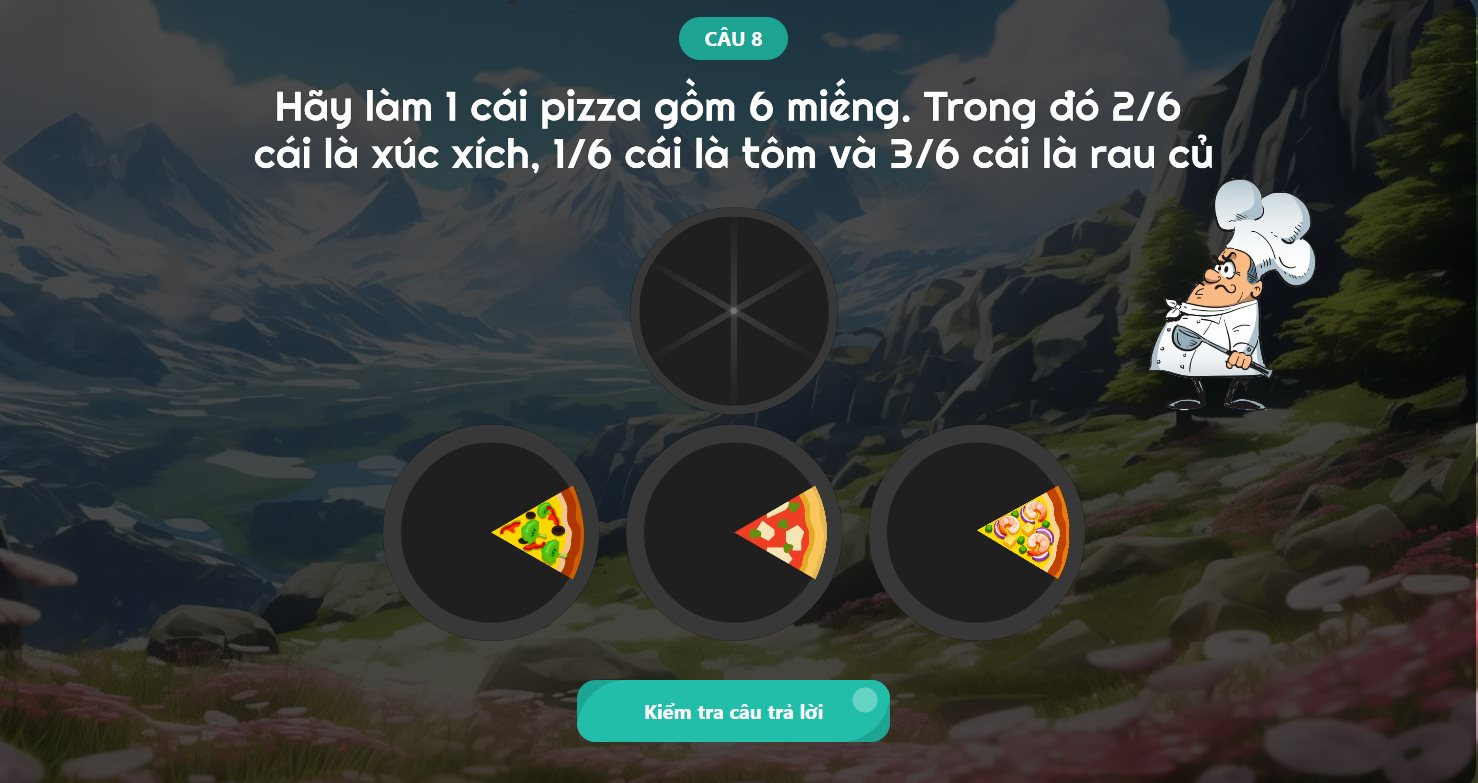
\includegraphics[width=0.9\textwidth]{Image/UI/Exercises/Pizza.jpg}
	\caption{Dạng bài chia pizza}
	\label{fig:pizza}
\end{figure}

\subsubsubsection{Thả chim (Release Bird)}
Dạng bài thả chim có cơ chế tương tự bài trắc nghiệm nhưng được thiết kế với phong cách tương tác sinh động hơn dành cho học sinh lớp nhỏ. Mỗi đáp án được biểu diễn bằng một chiếc lồng chim, phía dưới có bảng hiển thị nội dung đáp án tương ứng. Khi người học chọn đáp án, chiếc lồng sẽ rơi xuống và mở ra để chú chim bay đi, tạo cảm giác vui nhộn và tăng hứng thú học tập.

\begin{figure}[H]
	\centering
	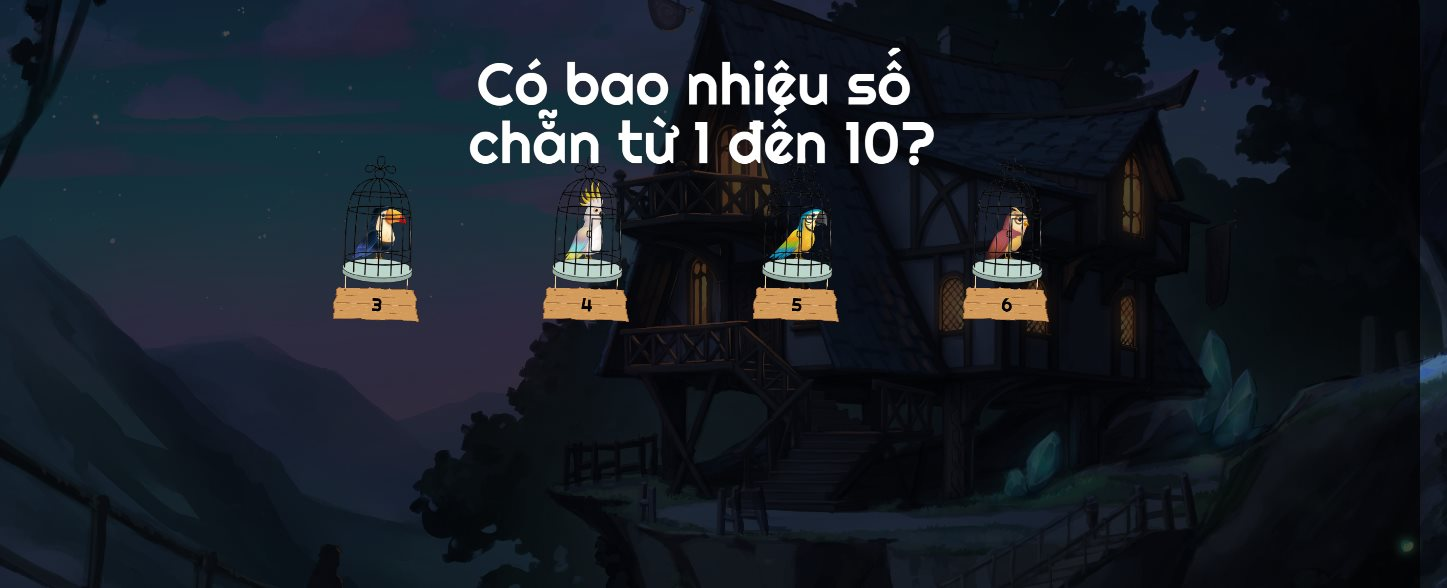
\includegraphics[width=0.9\textwidth]{Image/UI/Exercises/RealeaseBirt.jpg}
	\caption{Dạng bài thả chim}
	\label{fig:release-bird}
\end{figure}

\subsubsubsection{Cân điện tử (Scale)}
Dạng bài cân điện tử yêu cầu học sinh lựa chọn các quả tạ có giá trị khác nhau để đạt đúng khối lượng mục tiêu được đề bài đưa ra. Người học sẽ kéo các quả tạ lên bàn cân và hệ thống sẽ tự động tính tổng khối lượng hiện tại. Một bài toán có thể tồn tại nhiều cách chọn tạ khác nhau miễn tổng khối lượng đạt đúng yêu cầu.

\begin{figure}[H]
	\centering
	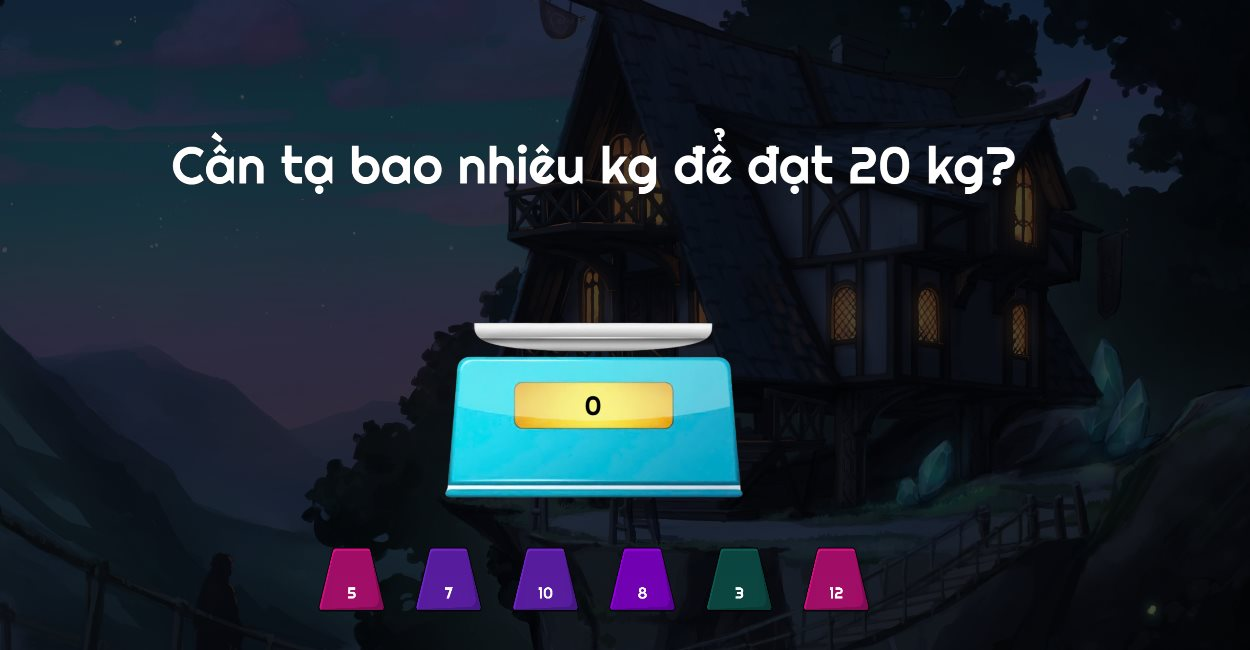
\includegraphics[width=0.9\textwidth]{Image/UI/Exercises/Scale.jpg}
	\caption{Dạng bài cân điện tử}
	\label{fig:scale}
\end{figure}

\subsubsubsection{Tưới cây (Tree)}
Dạng bài tưới cây gồm năm giai đoạn phát triển của cây tương ứng với năm câu hỏi liên tiếp. Mỗi khi trả lời đúng, mây sẽ xuất hiện và tạo mưa giúp cây phát triển sang giai đoạn tiếp theo. Nếu trả lời sai, cây sẽ quay trở lại trạng thái trước đó. Đáp án của mỗi câu hỏi được biểu diễn bằng số lần nhấn nút tương tác. Ví dụ, với bài toán \(2 + X = 5\), học sinh cần nhấn nút ba lần để tạo ra đáp án đúng.

\begin{figure}[H]
	\centering
	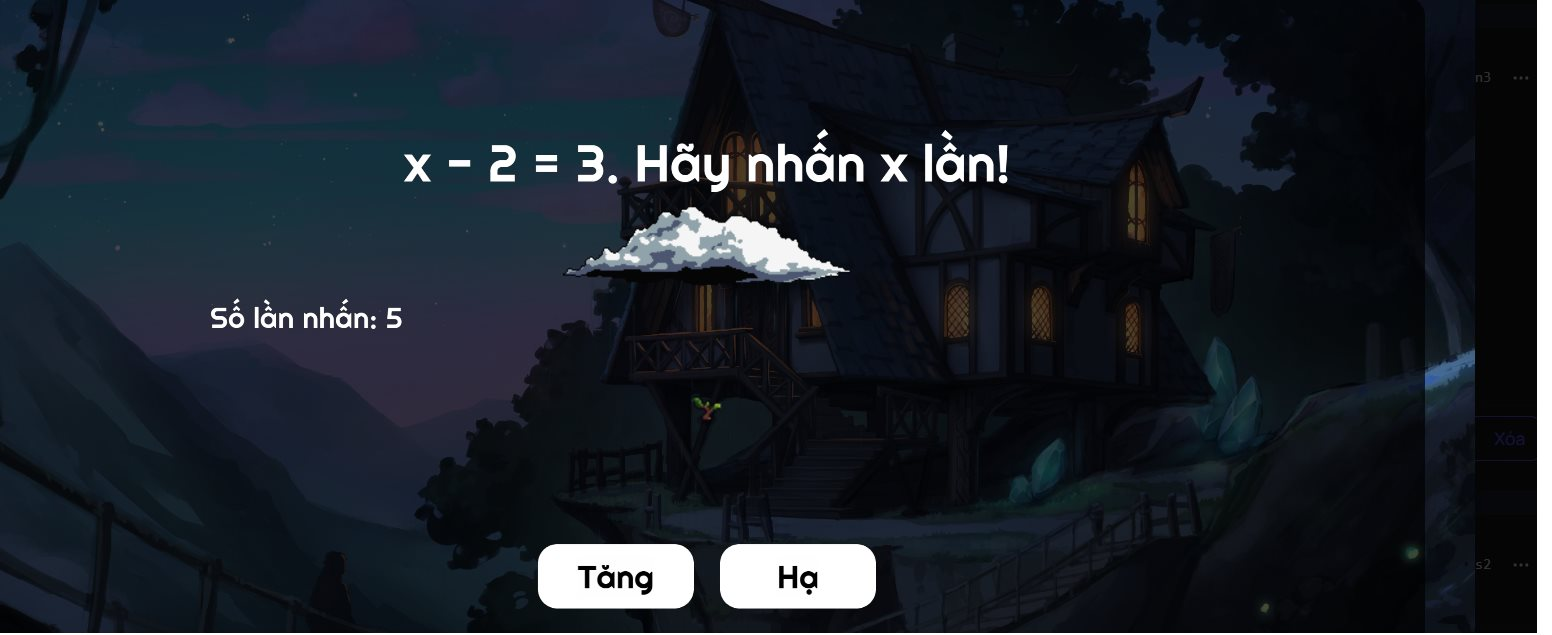
\includegraphics[width=0.9\textwidth]{Image/UI/Exercises/Tree.jpg}
	\caption{Dạng bài tưới cây}
	\label{fig:tree}
\end{figure}

\subsubsubsection{Vẽ hình (Geo)}
Dạng bài vẽ hình được xây dựng theo cơ chế tương tự geoboard. Người học có thể chọn các điểm cố định trên bảng và kéo nối để tạo thành các hình học khác nhau. Hệ thống hỗ trợ nhiều cách vẽ khác nhau cho cùng một đáp án, giúp tăng tính sáng tạo và khả năng tư duy hình học của học sinh.

\begin{figure}[H]
	\centering
	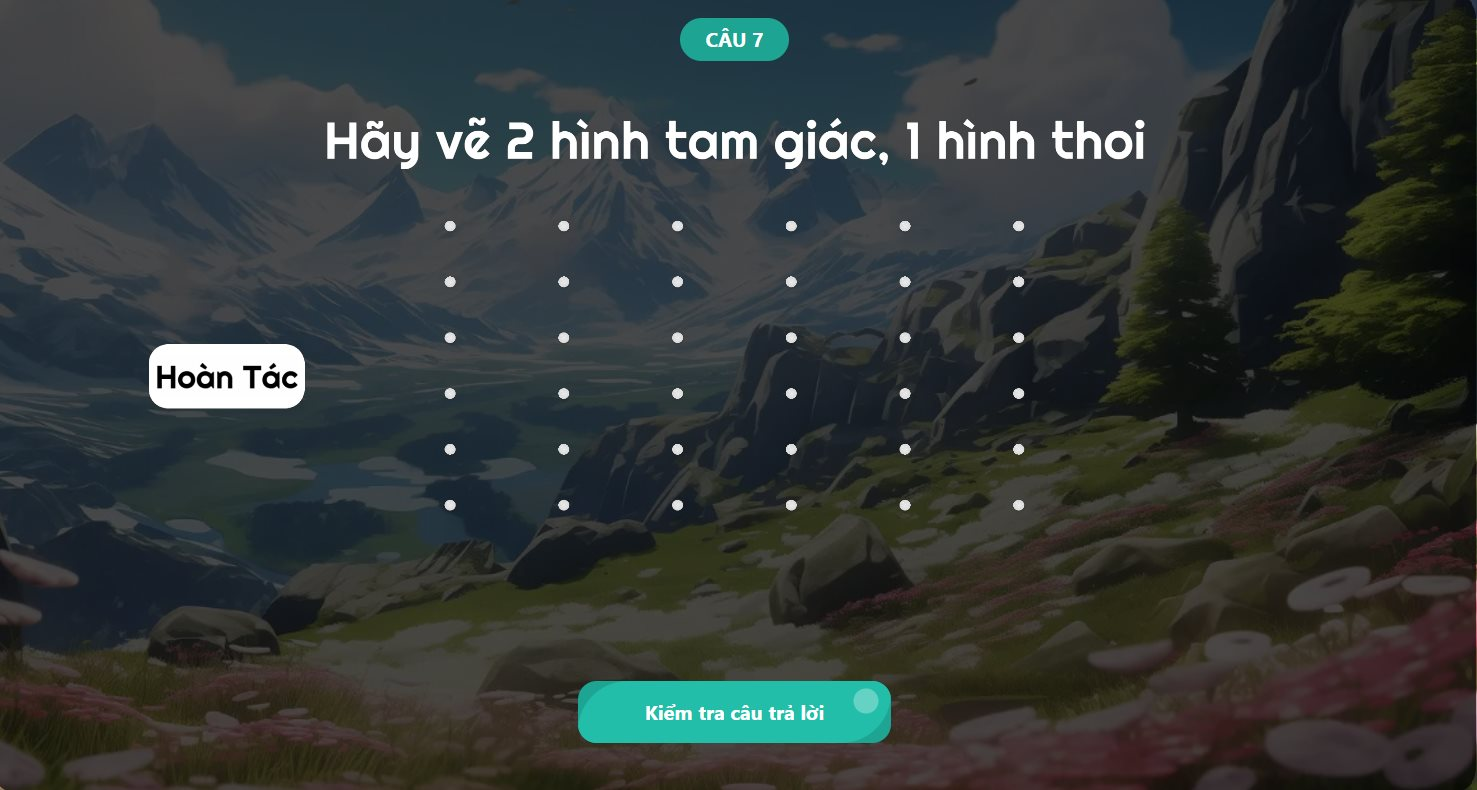
\includegraphics[width=0.9\textwidth]{Image/UI/Exercises/Geo.jpg}
	\caption{Dạng bài vẽ hình}
	\label{fig:geo}
\end{figure}

\subsubsection{Cơ sở học thuật xây dựng bài tập}

Nội dung các bài tập trong hệ thống được xây dựng dựa trên chương trình giáo dục môn Toán cấp Tiểu học của Bộ Giáo dục và Đào tạo. Mỗi chủ đề được phân chia theo ba mức độ nhận thức: \textbf{Nhận biết} (ghi nhớ, tái hiện thông tin), \textbf{Thông hiểu} (giải thích, áp dụng trực tiếp) và \textbf{Vận dụng} (phân tích, giải quyết vấn đề trong tình huống thực tế), nhằm đảm bảo tính phân hóa và phù hợp với từng trình độ học sinh.

% ===================== LỚP 1 =====================
\newpage
\paragraph{Lớp 1}
\renewcommand{\arraystretch}{1.3}
\begin{longtable}{|>{\centering\arraybackslash}m{0.8cm}|m{3.5cm}|>{\centering\arraybackslash}m{2cm}|m{7.5cm}|}
	\hline
	\textbf{STT} & \textbf{Chủ đề} & \textbf{Mức độ} & \textbf{Ví dụ minh họa} \\
	\hline
	\endfirsthead
	\hline
	\textbf{STT} & \textbf{Chủ đề} & \textbf{Mức độ} & \textbf{Ví dụ minh họa} \\
	\hline
	\endhead
	\hline
	\endfoot

	1 & Các số đến 10 và các phép tính cơ bản
	& Nhận biết & Viết các số từ 1 đến 10. (Ví dụ: Viết số 7) \\
	\cline{3-4}
	& & Thông hiểu & Thực hiện phép cộng/trừ đơn giản. ($5+3=?$ hoặc $8-2=?$) \\
	\cline{3-4}
	& & Vận dụng & Giải bài toán có lời văn. (Bạn An có 6 cái kẹo, mẹ cho thêm 4 cái. Hỏi An có tất cả bao nhiêu cái kẹo?) \\
	\hline

	2 & So sánh và các dấu toán học
	& Nhận biết & So sánh số lượng đồ vật. (Nhóm nào nhiều hơn, nhóm nào ít hơn?) \\
	\cline{3-4}
	& & Thông hiểu & Điền dấu thích hợp. ($5 \ldots 9$, điền dấu $<$, $>$, $=$ vào chỗ trống) \\
	\cline{3-4}
	& & Vận dụng & So sánh thực tế. (Bạn Lan có 7 viên bi, bạn Nam có 10 viên bi. Ai có nhiều hơn và nhiều hơn mấy viên?) \\
	\hline

	3 & Hình học cơ bản
	& Nhận biết & Chỉ ra các hình đã học. (Trong các hình sau, đâu là hình tam giác?) \\
	\cline{3-4}
	& & Thông hiểu & Đếm số lượng hình. (Trong hình vẽ này có bao nhiêu hình vuông?) \\
	\cline{3-4}
	& & Vận dụng & Ghép hình để tạo hình mới. (Ghép 2 hình tam giác lại, em được hình gì?) \\
	\hline

	4 & Vị trí và phương hướng
	& Nhận biết & Xác định vị trí. (Con mèo đang ở trên hay dưới cái ghế?) \\
	\cline{3-4}
	& & Thông hiểu & Mô tả vị trí của vật. (Con chim đang bay bên trái cái cây.) \\
	\cline{3-4}
	& & Vận dụng & Vẽ một quả bóng bên phải cái hộp và một bông hoa bên trên quả bóng. \\
	\hline

	5 & Các số có hai chữ số
	& Nhận biết & Viết số có hai chữ số. (Viết số "hai mươi lăm".) \\
	\cline{3-4}
	& & Thông hiểu & Phân tích cấu tạo số. (Trong số 37, số 3 thuộc hàng gì, số 7 thuộc hàng gì?) \\
	\cline{3-4}
	& & Vận dụng & Sắp xếp các số 25, 18, 32, 9 theo thứ tự từ bé đến lớn. \\
	\hline

	6 & Phép cộng, trừ trong phạm vi 100 (không nhớ)
	& Nhận biết & Thực hiện phép tính. ($23+6=?$ hoặc $45-20=?$) \\
	\cline{3-4}
	& & Thông hiểu & Điền số còn thiếu. ($40 + \ldots = 47$) \\
	\cline{3-4}
	& & Vận dụng & Bạn có 28 cái nhãn vở, mua thêm 11 cái. Hỏi bạn có tất cả bao nhiêu cái nhãn vở? \\
	\hline

	7 & Phép cộng, trừ có nhớ trong phạm vi 100
	& Nhận biết & Thực hiện phép tính. ($8+7=?$ hoặc $15-9=?$) \\
	\cline{3-4}
	& & Thông hiểu & Đặt tính rồi tính $19+24$ và $52-18$. \\
	\cline{3-4}
	& & Vận dụng & Lớp 1A có 24 học sinh, lớp 1B có 29 học sinh. Cả hai lớp có bao nhiêu học sinh? \\
	\hline

	8 & Đo lường cơ bản
	& Nhận biết & Dùng thước kẻ đo độ dài của một cây bút chì. \\
	\cline{3-4}
	& & Thông hiểu & An đo bàn được 5 gang, Bình đo được 6 gang. Bàn tay của ai lớn hơn? \\
	\cline{3-4}
	& & Vận dụng & Một sợi dây dài 20 cm, cắt đi 8 cm. Sợi dây còn lại dài bao nhiêu cm? \\
	\hline

	9 & Thời gian và xem đồng hồ
	& Nhận biết & Xem giờ đúng. (Đồng hồ chỉ mấy giờ?) \\
	\cline{3-4}
	& & Thông hiểu & An ăn sáng lúc 7 giờ, đi học lúc 8 giờ. Hoạt động nào diễn ra trước? \\
	\cline{3-4}
	& & Vận dụng & Bây giờ là 10 giờ. Sau 3 tiếng nữa sẽ là mấy giờ? \\
	\hline

	10 & Giải bài toán có lời văn
	& Nhận biết & Tóm tắt bài toán. (Có 5 con chim, 2 con bay đi. Còn lại bao nhiêu con? $5-2=?$) \\
	\cline{3-4}
	& & Thông hiểu & Có 5 quả táo trong giỏ, mẹ bỏ thêm 3 quả. Giỏ có bao nhiêu quả? \\
	\cline{3-4}
	& & Vận dụng & Nhà Mai có 10 con gà, bán 4 con, rồi mua thêm 2 con. Còn lại bao nhiêu con gà? \\
	\hline

	\caption{Các chủ đề toán lớp 1 theo chương trình Bộ GD\&ĐT}
	\label{tab:toan-lop1}
\end{longtable}

% ===================== LỚP 2 =====================
\paragraph{Lớp 2}
\renewcommand{\arraystretch}{1.3}
\begin{longtable}{|>{\centering\arraybackslash}m{0.8cm}|m{3.5cm}|>{\centering\arraybackslash}m{2cm}|m{7.5cm}|}
	\hline
	\textbf{STT} & \textbf{Chủ đề} & \textbf{Mức độ} & \textbf{Ví dụ minh họa} \\
	\hline
	\endfirsthead
	\hline
	\textbf{STT} & \textbf{Chủ đề} & \textbf{Mức độ} & \textbf{Ví dụ minh họa} \\
	\hline
	\endhead
	\hline
	\endfoot

	1 & Ôn tập phép cộng, trừ (có nhớ) trong phạm vi 100
	& Nhận biết & Thực hiện phép tính: $12+8=?$ \\
	\cline{3-4}
	& & Thông hiểu & Đặt tính rồi tính: $34+48$. \\
	\cline{3-4}
	& & Vận dụng & Một cửa hàng bán được 45 chiếc bánh mì buổi sáng, buổi chiều bán thêm 37 chiếc. Hỏi cả ngày bán được bao nhiêu chiếc? \\
	\hline

	2 & Cấu tạo phép tính
	& Nhận biết & Trong phép tính $25+13=38$, hãy chỉ ra số hạng và tổng. \\
	\cline{3-4}
	& & Thông hiểu & Phép tính $50-20=30$: đâu là số bị trừ, số trừ và hiệu? \\
	\cline{3-4}
	& & Vận dụng & Tìm số hạng còn thiếu: $15 + \ldots = 40$. \\
	\hline

	3 & Các số trong phạm vi 1\,000
	& Nhận biết & Đọc số 453. \\
	\cline{3-4}
	& & Thông hiểu & Viết số có hàng trăm là 2, hàng chục là 5, hàng đơn vị là 9. \\
	\cline{3-4}
	& & Vận dụng & Sắp xếp các số 325, 253, 532 theo thứ tự từ bé đến lớn. \\
	\hline

	4 & Phép cộng, trừ trong phạm vi 1\,000
	& Nhận biết & Thực hiện phép tính: $200+50=?$ \\
	\cline{3-4}
	& & Thông hiểu & Đặt tính rồi tính: $435+287$. \\
	\cline{3-4}
	& & Vận dụng & Thư viện có 560 quyển sách, nhà trường mua thêm 250 quyển. Hỏi thư viện có tất cả bao nhiêu quyển? \\
	\hline

	5 & Phép nhân và bảng nhân
	& Nhận biết & Chuyển phép cộng $2+2+2+2$ thành phép nhân. \\
	\cline{3-4}
	& & Thông hiểu & Tính tích của $5 \times 6$. \\
	\cline{3-4}
	& & Vận dụng & Mỗi bạn được phát 5 quyển vở. Hỏi 4 bạn sẽ nhận được bao nhiêu quyển vở? \\
	\hline

	6 & Phép chia và bảng chia
	& Nhận biết & Thực hiện phép chia: $10:2=?$ \\
	\cline{3-4}
	& & Thông hiểu & Phép tính nào đúng? (A) $10:5=2$ hoặc (B) $10:2=5$. \\
	\cline{3-4}
	& & Vận dụng & Có 25 cái kẹo, chia đều cho 5 bạn. Hỏi mỗi bạn được bao nhiêu cái kẹo? \\
	\hline

	7 & Đo lường (Độ dài và Khối lượng)
	& Nhận biết & Đọc và viết các đơn vị đo: 1 kg, 1 m, 1 dm. \\
	\cline{3-4}
	& & Thông hiểu & Đổi đơn vị đo: $1\,\text{m} = \ldots\,\text{dm}$. \\
	\cline{3-4}
	& & Vận dụng & Một khúc gỗ dài 20 m, người ta cưa đi 8 m. Hỏi khúc gỗ còn lại dài bao nhiêu mét? \\
	\hline

	8 & Hình học và đo lường
	& Nhận biết & Chỉ ra đâu là đường thẳng, đường cong, đường gấp khúc. \\
	\cline{3-4}
	& & Thông hiểu & Đo độ dài một đoạn thẳng bằng thước kẻ. \\
	\cline{3-4}
	& & Vận dụng & Tính độ dài đường gấp khúc gồm 3 đoạn thẳng dài lần lượt 20 cm, 15 cm, 10 cm. \\
	\hline

	9 & Thời gian và tiền tệ
	& Nhận biết & Xem đồng hồ chỉ 9 giờ 15 phút. \\
	\cline{3-4}
	& & Thông hiểu & Hôm nay là thứ ba. Hỏi ngày mai là thứ mấy? \\
	\cline{3-4}
	& & Vận dụng & Bây giờ là 8 giờ. Sau 15 phút nữa sẽ là mấy giờ? \\
	\hline

	10 & Thống kê và xác suất
	& Nhận biết & Biểu đồ tranh dưới đây cho biết có bao nhiêu quả táo? \\
	\cline{3-4}
	& & Thông hiểu & Lập bảng kiểm đếm số lượng bạn trai, bạn gái trong lớp. \\
	\cline{3-4}
	& & Vận dụng & Gieo một con xúc xắc: chắc chắn, có thể hay không thể ra mặt có 7 chấm? \\
	\hline

	\caption{Các chủ đề toán lớp 2 theo chương trình Bộ GD\&ĐT}
	\label{tab:toan-lop2}
\end{longtable}

% ===================== LỚP 3 =====================
\paragraph{Lớp 3}
\renewcommand{\arraystretch}{1.3}
\begin{longtable}{|>{\centering\arraybackslash}m{0.8cm}|m{3.5cm}|>{\centering\arraybackslash}m{2cm}|m{7.5cm}|}
	\hline
	\textbf{STT} & \textbf{Chủ đề} & \textbf{Mức độ} & \textbf{Ví dụ minh họa} \\
	\hline
	\endfirsthead
	\hline
	\textbf{STT} & \textbf{Chủ đề} & \textbf{Mức độ} & \textbf{Ví dụ minh họa} \\
	\hline
	\endhead
	\hline
	\endfoot

	1 & Hoàn thiện bảng nhân, bảng chia
	& Nhận biết & $7 \times 8 = ?$ \\
	\cline{3-4}
	& & Thông hiểu & Tìm số bị chia trong phép chia: $\ldots : 4 = 9$. \\
	\cline{3-4}
	& & Vận dụng & Có 35 bông hoa, cắm vào các lọ, mỗi lọ 5 bông. Hỏi cắm được bao nhiêu lọ hoa? \\
	\hline

	2 & Phân số cơ bản
	& Nhận biết & Tô màu vào $\dfrac{1}{3}$ hình tròn sau. \\
	\cline{3-4}
	& & Thông hiểu & Sắp xếp các phân số theo thứ tự từ bé đến lớn: $\dfrac{1}{2}$, $\dfrac{1}{4}$, $\dfrac{1}{3}$. \\
	\cline{3-4}
	& & Vận dụng & Mẹ có 12 quả cam, cho An $\dfrac{1}{4}$ số cam đó. Hỏi mẹ đã cho An bao nhiêu quả cam? \\
	\hline

	3 & Các số trong phạm vi 100\,000
	& Nhận biết & Viết số "mười hai nghìn không trăm năm mươi tư". \\
	\cline{3-4}
	& & Thông hiểu & Phân tích cấu tạo số: 45\,782 gồm bao nhiêu nghìn, trăm, chục, đơn vị? \\
	\cline{3-4}
	& & Vận dụng & Sắp xếp các số 23\,456; 23\,546; 23\,465 theo thứ tự từ lớn đến bé. \\
	\hline

	4 & Cộng, trừ, nhân, chia trong phạm vi 100\,000
	& Nhận biết & $25\,431 + 10\,520 = ?$ \\
	\cline{3-4}
	& & Thông hiểu & Đặt tính rồi tính $15\,328 \times 4$ và $48\,576 : 6$. \\
	\cline{3-4}
	& & Vận dụng & Một xưởng may sản xuất 12\,560 chiếc áo tháng đầu, tháng thứ hai sản xuất nhiều hơn 2\,500 chiếc. Hỏi cả hai tháng sản xuất được bao nhiêu chiếc? \\
	\hline

	5 & Tìm thành phần chưa biết của phép tính
	& Nhận biết & Tìm $x$ trong phép tính $x + 15 = 20$. \\
	\cline{3-4}
	& & Thông hiểu & Tìm $x$ trong phép tính $x : 7 = 8$. \\
	\cline{3-4}
	& & Vận dụng & Tìm $x$ trong phép tính $100 - x = 25 \times 3$. \\
	\hline

	6 & Giải toán với biểu thức và hai bước tính
	& Nhận biết & Tính giá trị của biểu thức: $500 + 50 \times 2$. \\
	\cline{3-4}
	& & Thông hiểu & An có 20 viên bi, Bình có gấp 3 lần số bi của An. Hỏi Bình có bao nhiêu viên bi? \\
	\cline{3-4}
	& & Vận dụng & Một cửa hàng có 500 kg gạo tẻ, đã bán 250 kg và còn lại $\dfrac{1}{2}$ số gạo đã bán. Hỏi ban đầu cửa hàng có bao nhiêu kg gạo? \\
	\hline

	7 & Hình học cơ bản
	& Nhận biết & Đâu là góc vuông, đâu là góc không vuông? \\
	\cline{3-4}
	& & Thông hiểu & Vẽ một đoạn thẳng AB dài 5 cm. \\
	\cline{3-4}
	& & Vận dụng & Vẽ một hình chữ nhật có chiều dài 8 cm và chiều rộng 5 cm. \\
	\hline

	8 & Chu vi và diện tích
	& Nhận biết & Tính chu vi của hình vuông có cạnh dài 5 cm. \\
	\cline{3-4}
	& & Thông hiểu & Tính diện tích của hình chữ nhật có chiều dài 10 cm và chiều rộng 6 cm. \\
	\cline{3-4}
	& & Vận dụng & Một mảnh vườn hình chữ nhật dài 20 m, rộng 15 m. Người ta rào lưới xung quanh. Hỏi cần bao nhiêu mét lưới? \\
	\hline

	9 & Đo lường (Độ dài, khối lượng, dung tích, nhiệt độ)
	& Nhận biết & Viết ký hiệu của đơn vị đo: mililitre. \\
	\cline{3-4}
	& & Thông hiểu & Đổi đơn vị: $3\,\text{kg} = \ldots\,\text{g}$. \\
	\cline{3-4}
	& & Vận dụng & Một xe tải chở 1\,500 kg gạo và thêm 500 kg ngô. Hỏi xe tải chở tất cả bao nhiêu tạ? (biết $1\,\text{tạ} = 100\,\text{kg}$) \\
	\hline

	10 & Thống kê và xác suất
	& Nhận biết & Theo biểu đồ, lớp 2 có bao nhiêu học sinh? \\
	\cline{3-4}
	& & Thông hiểu & Lập bảng thống kê số lượng các loại quả: 3 quả táo, 2 quả cam, 4 quả dứa. \\
	\cline{3-4}
	& & Vận dụng & Khi gieo một đồng xu, khả năng nào sẽ xảy ra: chắc chắn ra mặt sấp, có thể ra mặt sấp, hay không thể ra mặt sấp? \\
	\hline

	\caption{Các chủ đề toán lớp 3 theo chương trình Bộ GD\&ĐT}
	\label{tab:toan-lop3}
\end{longtable}

% ===================== LỚP 4 =====================
\paragraph{Lớp 4}
\renewcommand{\arraystretch}{1.3}
\begin{longtable}{|>{\centering\arraybackslash}m{0.8cm}|m{3.5cm}|>{\centering\arraybackslash}m{2cm}|m{7.5cm}|}
	\hline
	\textbf{STT} & \textbf{Chủ đề} & \textbf{Mức độ} & \textbf{Ví dụ minh họa} \\
	\hline
	\endfirsthead
	\hline
	\textbf{STT} & \textbf{Chủ đề} & \textbf{Mức độ} & \textbf{Ví dụ minh họa} \\
	\hline
	\endhead
	\hline
	\endfoot

	1 & Các số tự nhiên có nhiều chữ số
	& Nhận biết & Đọc và viết số có nhiều chữ số. (Ví dụ: "một trăm hai mươi ba triệu...") \\
	\cline{3-4}
	& & Thông hiểu & Xác định giá trị vị trí. (Ví dụ: Chữ số 5 trong 123\,456\,789 có giá trị là 500\,000.) \\
	\cline{3-4}
	& & Vận dụng & So sánh và sắp xếp các số có nhiều chữ số theo thứ tự. \\
	\hline

	2 & Các phép tính với số tự nhiên
	& Nhận biết & Thực hiện bốn phép tính cơ bản với các số lớn, kể cả phép chia có dư. \\
	\cline{3-4}
	& & Thông hiểu & Vận dụng tính chất giao hoán, kết hợp để tính nhẩm nhanh. (Ví dụ: $25 \times 36 \times 4$) \\
	\cline{3-4}
	& & Vận dụng & Tìm số bị chia, số chia trong phép chia có dư. \\
	\hline

	3 & Số trung bình cộng
	& Nhận biết & Nắm vững công thức tính trung bình cộng. \\
	\cline{3-4}
	& & Thông hiểu & Tính trung bình cộng của dãy số: 10, 20, 30, 40. \\
	\cline{3-4}
	& & Vận dụng & Một đội ngày đầu trồng 200 cây, ngày thứ hai trồng 300 cây. Trung bình mỗi ngày trồng được bao nhiêu cây? \\
	\hline

	4 & Phân số và các phép tính cơ bản
	& Nhận biết & Nhận biết khái niệm phân số: tử số, mẫu số. \\
	\cline{3-4}
	& & Thông hiểu & Rút gọn phân số và quy đồng mẫu số. \\
	\cline{3-4}
	& & Vận dụng & So sánh các phân số khác mẫu số. \\
	\hline

	5 & Các phép tính với phân số
	& Nhận biết & Cộng, trừ, nhân, chia phân số cùng mẫu số. \\
	\cline{3-4}
	& & Thông hiểu & Cộng, trừ phân số khác mẫu số sau khi quy đồng. \\
	\cline{3-4}
	& & Vận dụng & Một tấm vải dài $\frac{3}{4}$ m, cắt đi $\frac{1}{2}$ m. Hỏi tấm vải còn lại dài bao nhiêu mét? \\
	\hline

	6 & Hình học cơ bản
	& Nhận biết & Nhận biết và gọi tên hình bình hành, hình thoi. \\
	\cline{3-4}
	& & Thông hiểu & Phân biệt góc nhọn, góc tù, góc bẹt; đường thẳng vuông góc, song song. \\
	\cline{3-4}
	& & Vận dụng & Vẽ hình theo yêu cầu. \\
	\hline

	7 & Chu vi và diện tích
	& Nhận biết & Công thức tính chu vi và diện tích hình vuông, hình chữ nhật. \\
	\cline{3-4}
	& & Thông hiểu & Chuyển đổi đơn vị đo diện tích (m$^2$, dm$^2$). \\
	\cline{3-4}
	& & Vận dụng & Tính chu vi và diện tích trong tình huống thực tế, kể cả bài toán ghép hình. \\
	\hline

	8 & Đo lường (Khối lượng và thời gian)
	& Nhận biết & Các đơn vị đo khối lượng lớn: yến, tạ, tấn; thời gian: thế kỷ, giây. \\
	\cline{3-4}
	& & Thông hiểu & Chuyển đổi đơn vị. (Ví dụ: $1\,\text{tấn} = \ldots\,\text{kg}$) \\
	\cline{3-4}
	& & Vận dụng & Một xe tải chở 5 tấn hàng, đã dỡ 2 tạ. Trên xe còn lại bao nhiêu kg hàng? \\
	\hline

	9 & Thống kê và biểu đồ
	& Nhận biết & Đọc và hiểu thông tin từ biểu đồ cột. \\
	\cline{3-4}
	& & Thông hiểu & Lập bảng thống kê từ một dãy số liệu. \\
	\cline{3-4}
	& & Vận dụng & Phân tích biểu đồ: lớp nào có nhiều học sinh giỏi nhất? \\
	\hline

	10 & Toán nâng cao và biểu thức
	& Nhận biết & Bài toán tìm hai số khi biết tổng và hiệu. \\
	\cline{3-4}
	& & Thông hiểu & Tính giá trị biểu thức: $a + b \times 5$ khi $a=10$, $b=2$. \\
	\cline{3-4}
	& & Vận dụng & Bài toán rút về đơn vị. (Ví dụ: 3 kg táo hết 60\,000 đồng. Hỏi 5 kg hết bao nhiêu tiền?) \\
	\hline

	\caption{Các chủ đề toán lớp 4 theo chương trình Bộ GD\&ĐT}
	\label{tab:toan-lop4}
\end{longtable}

% ===================== LỚP 5 =====================
\paragraph{Lớp 5}
\renewcommand{\arraystretch}{1.3}
\begin{longtable}{|>{\centering\arraybackslash}m{0.8cm}|m{3.5cm}|>{\centering\arraybackslash}m{2cm}|m{7.5cm}|}
	\hline
	\textbf{STT} & \textbf{Chủ đề} & \textbf{Mức độ} & \textbf{Ví dụ minh họa} \\
	\hline
	\endfirsthead
	\hline
	\textbf{STT} & \textbf{Chủ đề} & \textbf{Mức độ} & \textbf{Ví dụ minh họa} \\
	\hline
	\endhead
	\hline
	\endfoot

	1 & Ôn tập và bổ sung kiến thức
	& Nhận biết & Một đội công nhân sửa đường, ngày đầu sửa được 120 m, ngày thứ hai sửa nhiều hơn ngày đầu 15 m. Hỏi ngày thứ hai sửa được bao nhiêu mét đường? \\
	\cline{3-4}
	& & Thông hiểu & Một tấm vải dài 30 m, đã bán được $\dfrac{2}{3}$ tấm vải. Hỏi còn lại bao nhiêu mét vải? \\
	\cline{3-4}
	& & Vận dụng & Một cửa hàng bán gạo buổi sáng 500 kg, buổi chiều bán $\dfrac{1}{2}$ số gạo buổi sáng. Hỏi cả hai buổi cửa hàng bán được bao nhiêu tạ gạo? \\
	\hline

	2 & Số thập phân
	& Nhận biết & Viết các số: "Năm phẩy bảy mươi lăm" và "Bốn trăm năm mươi sáu phẩy không không tám". \\
	\cline{3-4}
	& & Thông hiểu & Sắp xếp theo thứ tự từ lớn đến bé: 12,3; 12,03; 12,31; 12,13. \\
	\cline{3-4}
	& & Vận dụng & Dùng 3 chữ số 0, 5, 8 và dấu phẩy, hãy viết tất cả các số thập phân có hai chữ số ở phần thập phân và lớn hơn 50. \\
	\hline

	3 & Các phép tính với số thập phân
	& Nhận biết & Thực hiện phép tính: $15{,}4 + 8{,}9 = ?$ \\
	\cline{3-4}
	& & Thông hiểu & Mẹ mua cá hết 56\,500 đồng và mua rau hết 15\,500 đồng, đưa 100\,000 đồng. Hỏi mẹ được trả lại bao nhiêu tiền? \\
	\cline{3-4}
	& & Vận dụng & Một mảnh đất hình chữ nhật dài 25,5 m, chiều rộng bằng $\dfrac{2}{3}$ chiều dài. Tính chu vi và diện tích mảnh đất đó. \\
	\hline

	4 & Tỉ số và tỉ lệ
	& Nhận biết & Một lớp học có 20 bạn nam và 25 bạn nữ. Tìm tỉ số của số bạn nam và số bạn nữ. \\
	\cline{3-4}
	& & Thông hiểu & Lãi suất tiết kiệm là 0,5\% một tháng. Cô Lan gửi 10 triệu đồng. Hỏi sau một tháng cô nhận được bao nhiêu tiền lãi? \\
	\cline{3-4}
	& & Vận dụng & Tổng số tuổi của hai anh em là 36 tuổi. Tuổi em bằng $\dfrac{4}{5}$ tuổi anh. Tính tuổi của mỗi người. \\
	\hline

	5 & Hình học phẳng nâng cao
	& Nhận biết & Một hình tam giác có đáy 10 cm, chiều cao 8 cm. Tính diện tích hình tam giác đó. \\
	\cline{3-4}
	& & Thông hiểu & Một hình tròn có bán kính 5 dm. Tính chu vi và diện tích hình tròn đó. \\
	\cline{3-4}
	& & Vận dụng & Một mảnh đất hình thang có tổng độ dài hai đáy là 40 m, chiều cao 25 m. Tính diện tích mảnh đất. \\
	\hline

	6 & Hình học không gian cơ bản
	& Nhận biết & Một hình lập phương có cạnh 4 cm. Tính thể tích hình lập phương đó. \\
	\cline{3-4}
	& & Thông hiểu & Một hình hộp chữ nhật dài 12 m, rộng 8 m, cao 5 m. Tính diện tích xung quanh và diện tích toàn phần. \\
	\cline{3-4}
	& & Vận dụng & Một bể cá hình hộp chữ nhật dài 1,2 m, rộng 0,8 m, cao 1 m. Người ta đổ nước sao cho mực nước bằng $\dfrac{3}{4}$ chiều cao bể. Tính thể tích nước trong bể. \\
	\hline

	7 & Đo lường
	& Nhận biết & Đổi đơn vị: $12\,\text{tấn} = \ldots\,\text{kg}$. \\
	\cline{3-4}
	& & Thông hiểu & Một xe chở 5 tấn 50 kg gạo, lần đầu dỡ 2\,500 kg. Hỏi trên xe còn lại bao nhiêu tạ gạo? \\
	\cline{3-4}
	& & Vận dụng & Một ô tô đi từ A lúc 7 giờ 30 phút, đến B lúc 10 giờ 15 phút, dọc đường nghỉ 30 phút. Hỏi thời gian ô tô đi thực tế là bao lâu? \\
	\hline

	8 & Toán chuyển động đều
	& Nhận biết & Một người đi bộ vận tốc 5 km/giờ. Hỏi sau 2 giờ đi được bao nhiêu km? \\
	\cline{3-4}
	& & Thông hiểu & Một xe máy đi từ A đến B với vận tốc 40 km/giờ hết 2 giờ, sau đó quay về A với vận tốc 50 km/giờ. Tính thời gian xe đi từ B về A. \\
	\cline{3-4}
	& & Vận dụng & Hai ô tô khởi hành cùng lúc từ A và B (cách nhau 210 km) đi ngược chiều nhau. Vận tốc xe từ A là 50 km/giờ, xe từ B là 60 km/giờ. Hỏi sau bao lâu hai xe gặp nhau? \\
	\hline

	9 & Thống kê và xác suất
	& Nhận biết & Biểu đồ cho biết số học sinh thích môn bóng đá là bao nhiêu? \\
	\cline{3-4}
	& & Thông hiểu & Khối lớp 5 có 150 học sinh, trong đó 60 bạn nữ. Biểu diễn tỉ số phần trăm số bạn nữ và bạn nam bằng biểu đồ quạt. \\
	\cline{3-4}
	& & Vận dụng & Trong một hộp có 5 viên bi đỏ và 3 viên bi xanh. Không nhìn vào hộp, lấy ngẫu nhiên 1 viên. Việc lấy được bi đỏ có chắc chắn, có thể hay không thể xảy ra? \\
	\hline

	10 & Ứng dụng toán học vào thực tiễn
	& Nhận biết & Trên bản đồ tỉ lệ 1:1\,000, khoảng cách A và B là 5 cm. Hỏi khoảng cách thực tế là bao nhiêu mét? \\
	\cline{3-4}
	& & Thông hiểu & Một người gửi tiết kiệm 50 triệu đồng với lãi suất 0,6\% một tháng. Hỏi sau 2 tháng rút cả vốn lẫn lãi được bao nhiêu tiền? \\
	\cline{3-4}
	& & Vận dụng & Bác An mua tivi giá 10 triệu đồng, trả trước 40\%. Số còn lại trả góp trong 5 tháng đều nhau. Hỏi mỗi tháng bác phải trả bao nhiêu tiền? \\
	\hline

	\caption{Các chủ đề toán lớp 5 theo chương trình Bộ GD\&ĐT}
	\label{tab:toan-lop5}
\end{longtable}

\subsubsection{Ánh xạ dạng bài tập với chủ đề học thuật}

Bảng dưới đây thể hiện sự tương ứng giữa 18 dạng bài tập tương tác đã hiện thực và các chủ đề trong chương trình toán tiểu học. Ký hiệu \textbf{C\textit{n}} chỉ chủ đề thứ $n$ theo thứ tự trong bảng của từng lớp.

\renewcommand{\arraystretch}{1.35}
\begin{longtable}{|m{3.5cm}|>{\centering\arraybackslash}m{1.5cm}|>{\centering\arraybackslash}m{1.5cm}|>{\centering\arraybackslash}m{1.5cm}|>{\centering\arraybackslash}m{1.5cm}|>{\centering\arraybackslash}m{1.5cm}|m{3.5cm}|}
	\hline
	\textbf{Dạng bài tập} & \textbf{Lớp 1} & \textbf{Lớp 2} & \textbf{Lớp 3} & \textbf{Lớp 4} & \textbf{Lớp 5} & \textbf{Ghi chú} \\
	\hline
	\endfirsthead
	\hline
	\textbf{Dạng bài tập} & \textbf{Lớp 1} & \textbf{Lớp 2} & \textbf{Lớp 3} & \textbf{Lớp 4} & \textbf{Lớp 5} & \textbf{Ghi chú} \\
	\hline
	\endhead
	\hline
	\endfoot

	Trắc nghiệm \newline (Multiple Choice)
	& C1--C10 & C1--C10 & C1--C10 & C1--C10 & C1--C10
	& Áp dụng cho toàn bộ chủ đề \\
	\hline

	Ghép cặp \newline (Matching)
	& C2, C3 & C5, C6 & C1, C2 & C4, C6 & C4, C5
	& Ghép số, ghép hình, ghép phép tính tương đương \\
	\hline

	Điền số \newline (Fill in the Blanks)
	& C1, C6, C7 & C1, C2, C4 & C4, C5 & C2, C3 & C1, C3
	& Điền kết quả phép tính, tìm thành phần còn thiếu \\
	\hline

	Kéo thả \newline (Drag and Drop)
	& C1, C5 & C3, C4 & C3, C4 & C1, C2 & C2, C3
	& Điền số vào biểu thức, sắp xếp dãy số \\
	\hline

	Phân loại \newline (Grouping)
	& C1, C5 & C3 & C3 & C1 & C2
	& Phân loại chẵn/lẻ, phân loại hình, phân loại theo nhóm \\
	\hline

	Đúng/Sai \newline (True/False)
	& C2, C6, C7 & C1, C4, C5, C6 & C1, C4, C5 & C2, C4, C5 & C1, C3, C4
	& Kiểm tra tính đúng đắn của một phép tính hoặc mệnh đề so sánh \\
	\hline

	Tổ hợp Burger \newline (Burger)
	& -- & C10 & C10 & C10 & C9
	& Thống kê, xác suất tổ hợp \\
	\hline

	Xe buýt \newline (Bus)
	& C6 & C1, C4 & C4 & C2 & --
	& Cộng số tròn chục/tròn trăm; xếp hàng lên xe \\
	\hline

	Bắt chim \newline (Catch Bird)
	& C1, C6, C7 & C1, C4, C5 & C1, C4 & C2, C3 & C1, C3
	& Dạng tổng quát; biểu diễn nhiều dạng toán bằng cơ chế bắt chim \\
	\hline

	Đồng hồ \newline (Clock)
	& C9 & C9 & -- & C8 & C7
	& Đọc giờ kim, giờ số; tính thời gian \\
	\hline

	Đổi tiền xu \newline (Coin)
	& -- & C9 & -- & C8 & C10
	& Nhận biết mệnh giá, đổi tiền, tính toán với tiền tệ \\
	\hline

	Viên bi \newline (Gumball)
	& C1, C2 & C10 & C10 & C9 & C9
	& Đếm, so sánh số lượng; thống kê trực quan \\
	\hline

	Cân thủ công \newline (Manual Scale)
	& C2 & C7 & C9 & C8 & C7
	& So sánh lớn hơn/bé hơn/bằng nhau qua cân \\
	\hline

	Chia pizza \newline (Pizza)
	& -- & -- & C2 & C4, C5 & C4
	& Làm quen phân số, tỉ lệ qua hình ảnh trực quan \\
	\hline

	Thả chim \newline (Release Bird)
	& C1--C10 & C1--C10 & C1--C10 & C1--C10 & C1--C10
	& Áp dụng cho toàn bộ chủ đề \\
	\hline

	Cân điện tử \newline (Scale)
	& C6, C7 & C1, C4 & C4 & C2 & C3
	& Cộng/trừ qua cân bằng; có thể có nhiều đáp án đúng \\
	\hline

	Tưới cây \newline (Tree)
	& C10 & C2 & C6 & C10 & C10
	& Bài toán nhiều bước; tưới từng bước để hoàn thành \\
	\hline

	Vẽ hình \newline (Geo)
	& C3 & C8 & C7, C8 & C6, C7 & C5
	& Vẽ hình học; tính chu vi, diện tích \\
	\hline

	\caption{Ánh xạ giữa 18 dạng bài tập và chủ đề chương trình Bộ GD\&ĐT}
	\label{tab:exercise-mapping}
\end{longtable}

Kết quả phân tích bảng ánh xạ cho thấy hệ thống bài tập đạt được độ bao phủ toàn diện trên toàn bộ chương trình toán tiểu học. Với \textbf{18 dạng tương tác} được phân phối trải rộng qua \textbf{5 khối lớp} và \textbf{10 chủ đề học thuật} mỗi lớp, mọi đơn vị kiến thức trong chương trình của Bộ Giáo dục và Đào tạo đều có ít nhất một dạng bài tập phù hợp để luyện tập.
Điểm nhấn quan trọng trong thiết kế là hệ thống đề cao \textbf{tư duy linh hoạt}: nhiều dạng bài chấp nhận \textbf{nhiều cách giải khác nhau} miễn là kết quả cuối cùng là đúng, phản ánh đúng bản chất của toán học là khuyến khích học sinh tự tìm con đường tư duy của mình thay vì rập khuôn một đáp án duy nhất.
Ba mức độ nhận thức \textbf{Nhận biết -- Thông hiểu -- Vận dụng} được duy trì xuyên suốt theo đúng chuẩn chương trình của Bộ Giáo dục và Đào tạo, giúp hệ thống phục vụ toàn dải trình độ: từ học sinh mới làm quen khái niệm đến học sinh cần thử thách ở mức phân tích và giải quyết vấn đề thực tế. Sự kết hợp giữa độ bao phủ rộng theo chương trình, tính chuyên biệt theo từng miền kiến thức và triết lý tôn trọng tư duy đa hướng là nền tảng để hệ thống không chỉ dạy toán mà còn \textbf{rèn luyện cách suy nghĩ} cho học sinh tiểu học.